% ----------------------------------------------------------
% Desenvolvimento: requisitos, planejamento e arquitetura
% 
% ----------------------------------------------------------

\chapter[Desenvolvimento]{Desenvolvimento}

Este capítulo apresenta o desenvolvimento do MetaRefino, aplicativo para Windows destinado ao tratamento de matrizes de dados metabolômicos obtidas por cromatografia líquida acoplada à espectrometria de massas. São descritos o levantamento dos requisitos, a organização do projeto e a arquitetura que articula a interface gráfica, o processamento científico e a persistência. A exposição considera as necessidades relatadas pelo laboratório parceiro, as decisões registradas durante a implementação e as funcionalidades efetivamente acessíveis pelo fluxo principal da aplicação.

O escopo apresentado compreende a preparação dos arquivos, a validação, o diagnóstico, a correção do sinal, o pré-processamento, as análises estatísticas e a geração de resultados. Essa delimitação acompanha a adotada no capítulo de testes. A presença de uma implementação, por si só, não é tomada como comprovação de sua validação em todas as condições de uso.

A entrada do MetaRefino corresponde a uma matriz tabular já produzida pelo processamento primário, e não ao arquivo instrumental bruto. A detecção e o alinhamento dos picos permanecem no fluxo anterior, realizado com ferramentas como o Progenesis QI. Além disso, uma \textit{feature}, identificada por características do sinal como tempo de retenção e razão massa/carga, não equivale necessariamente a um metabólito identificado. O tratamento e as análises apresentados neste capítulo operam sobre essas variáveis e não estabelecem, isoladamente, a identidade química ou a relevância biológica de cada sinal.

A descrição da arquitetura e dos requisitos complementa a metodologia do capítulo anterior e antecede a apresentação do modelo de dados e da implementação nas seções seguintes. As evidências de funcionamento, as diferenças entre versões e as limitações das verificações são discutidas no capítulo de testes, especialmente nas Seções~\ref{sec:5-1-3} e~\ref{sec:5-5}.

\section{Levantamento e especificação dos requisitos}
\label{sec:4-requisitos}

Os requisitos foram organizados para relacionar as necessidades do laboratório às operações oferecidas pelo aplicativo e às verificações empregadas no desenvolvimento. A especificação contempla tanto os resultados esperados pelo pesquisador quanto as condições necessárias para produzir, interpretar e recuperar esses resultados. Assim, a correção numérica de uma operação é acompanhada por requisitos de validação da entrada, explicitação dos parâmetros, apresentação da qualidade e conservação do contexto da execução.

\subsection{Processo de levantamento dos requisitos}

O levantamento ocorreu por meio de reuniões presenciais e on-line, trocas de mensagens pelo WhatsApp, comunicações por e-mail e uma demonstração presencial no laboratório de metabolômica. Essas interações permitiram conhecer o fluxo de trabalho dos pesquisadores e discutir os arquivos utilizados, as dificuldades de preparação dos dados e as informações necessárias para avaliar um tratamento. A demonstração também forneceu um contexto de uso para discutir a organização da interface e o encadeamento das operações.

As informações obtidas foram complementadas pela análise das matrizes de medições, dos arquivos de descrição das amostras e dos procedimentos de referência em R disponibilizados ao projeto. Essa análise aproximou os relatos dos usuários das condições concretas de processamento: estrutura dos arquivos, representação das intensidades, identificação dos controles de qualidade, ordem de injeção e associação das amostras aos grupos experimentais. O arquivo de medições e sua lista de amostras passaram, dessa forma, a constituir uma entrada conjunta, cuja coerência precisa ser verificada antes do cálculo.

Entre as necessidades registradas encontra-se a preparação manual de matrizes em planilha para continuidade da análise em outras ferramentas. O relato estabelece a ocorrência desse procedimento, mas não permite afirmar sua frequência nem a inexistência de critérios informais. A resposta do projeto foi tornar explícitos os critérios aplicados pelo software e registrar as variáveis removidas na exportação, permitindo distinguir uma seleção executada pelo aplicativo de uma alteração sem registro do procedimento.

O refinamento dos requisitos acompanhou a implementação. A especificação foi decomposta em fases, com critérios de aceitação, e complementada por decisões técnicas e registros de divergências em relação ao processamento de referência. Posteriormente, os roteiros de teste do grupo relacionaram requisitos a cenários de utilização. Como as funcionalidades e a interface evoluíram após esses roteiros, a rastreabilidade precisa considerar a versão em que cada verificação foi realizada.

A formalização utilizou documentos com finalidades distintas. O documento de implementação reúne os contratos e os critérios de aceitação; o registro de decisões conserva as alterações e suas justificativas; o registro de divergências identifica diferenças em relação ao procedimento em R; e o registro de problemas de implementação conserva as situações que motivaram verificações adicionais. Essa organização permite acompanhar a evolução da solução sem interpretar uma descrição histórica como requisito vigente. Em particular, os primeiros desenhos de interface e os requisitos de funcionalidades posteriormente excluídas precisam ser lidos à luz das decisões de escopo.

Os arquivos analisados abrangem modos de aquisição que combinam polaridade positiva ou negativa com separação C18 ou HILIC. A especificação explicita essas condições, mas as observações obtidas nos conjuntos de referência não são tratadas como propriedades de qualquer estudo futuro. Quantidade de amostras, número de QCs e distribuição dos grupos são características da entrada e devem ser verificadas a cada carregamento.

\subsection{Atores e casos de uso}

O ator principal é o pesquisador ou analista do laboratório, responsável por selecionar os dados, avaliar as informações de diagnóstico, configurar o processamento e interpretar os resultados. A interface não estabelece perfis de autenticação distintos. Assim, pesquisador, avaliador e integrante do grupo que executa uma tarefa equivalente compartilham o mesmo fluxo operacional, ainda que tenham objetivos diferentes ao utilizar o aplicativo.

O operador da linha de comando constitui uma forma adicional de interação, voltada à execução por comandos e à repetição de procedimentos. O desenvolvedor atua na manutenção, na verificação e no empacotamento do software. O Progenesis QI é a ferramenta de origem dos arquivos tabulares, e o MetaboAnalyst é um possível destino dos arquivos exportados. Essas relações representam intercâmbio por arquivos; não significam integração automática com os dois programas.

Os principais casos de uso do fluxo entregue são os seguintes:
\begin{enumerate}
\item \textbf{Preparar e validar o estudo:} selecionar o par de arquivos e o modo de aquisição, verificar sua estrutura e examinar os erros e avisos encontrados.
\item \textbf{Diagnosticar os dados:} consultar indicadores de qualidade, indícios de variação técnica e propostas de organização dos lotes.
\item \textbf{Definir a correção:} aceitar o corretor que o palpite propõe, aplicado por padrão pela caixa ``Automático'', ou desmarcá-la, comparar os métodos disponíveis e selecionar o corretor que será aplicado.
\item \textbf{Executar o tratamento:} configurar e realizar a correção e o pré-processamento, pelo fluxo completo ou por etapas, com acompanhamento do trabalho.
\item \textbf{Avaliar os resultados:} consultar as métricas e as figuras correspondentes à matriz e ao estágio de processamento considerado.
\item \textbf{Obter os artefatos:} gerar e salvar as matrizes corrigida e processada e exportar a entrada compatível com o MetaboAnalyst.
\item \textbf{Interromper uma execução:} solicitar o cancelamento e acompanhar a transição do trabalho para seu estado terminal.
\end{enumerate}

No caso de uso de tratamento, os arquivos válidos e os parâmetros aceitos constituem as precondições. O fluxo principal envolve o envio da configuração, a execução das operações e a disponibilização dos resultados. Arquivos inconsistentes, parâmetros incompatíveis, cancelamento e falha de processamento constituem fluxos alternativos que precisam produzir uma indicação compreensível, sem apresentar uma saída parcial como resultado concluído.

A escolha da correção é apoiada pela comparação dos métodos disponíveis. O pesquisador pode solicitar a execução dos candidatos e examinar os resultados segundo o estimador definido. A comparação exige que os métodos sejam aplicáveis aos controles e aos lotes disponíveis e deve identificar o critério utilizado. Uma diferença de desempenho observada fornece um elemento para a decisão, sem determinar, por si só, qual procedimento deve ser adotado no estudo. A seleção final considera também as características dos dados e o julgamento metodológico do pesquisador.

Na exportação, a precondição é a existência de uma entrada e de uma configuração compatíveis com o formato solicitado. A pós-condição é a disponibilização do arquivo e do registro do recorte aplicado. O cancelamento antes da conclusão e a ausência de um artefato válido são fluxos alternativos; nesses casos, a interface deve informar o estado do trabalho e não oferecer o resultado como se estivesse concluído.

\subsection{Requisitos funcionais}

Os identificadores abaixo acompanham o levantamento relacionado ao plano de testes do grupo e utilizado no capítulo de testes. A numeração mantém lacunas correspondentes às funcionalidades excluídas, evitando atribuir um novo significado a identificadores já empregados nos registros do projeto.

\begin{description}
\item[RF-01 --- Seleção da entrada.] Permitir selecionar os arquivos de medições e de descrição das amostras e informar o modo de aquisição, distinguindo a finalidade de cada arquivo.
\item[RF-02 --- Validação.] Verificar a estrutura e a coerência da entrada, apresentar erros e avisos e impedir a continuidade quando houver condição incompatível com o processamento solicitado.
\item[RF-03 --- Diagnóstico.] Produzir um perfil dos dados e apresentar o diagnóstico e as propostas de fronteiras de lote, preservando a distinção entre indicação computacional e confirmação pelo pesquisador.
\item[RF-04 --- Apoio à escolha.] Propor o corretor por uma medição sobre a própria matriz e, por padrão, aplicá-lo pela caixa ``Automático''; permitir que o pesquisador a desmarque, compare os métodos de correção por meio de sua execução e da apresentação dos indicadores de qualidade e escolha o método a aplicar, identificando o critério empregado.
\item[RF-05 --- Correção.] Disponibilizar as opções \texttt{none}, \texttt{serrf} e \texttt{loess}. A primeira mantém o sinal sem correção e permite estabelecer uma condição de comparação.
\item[RF-06 --- Grupos experimentais.] Receber e validar o par de grupos utilizado nas análises que exigem essa definição, recusando referências a grupos inexistentes.
\item[RF-07 --- Validação do PLS-DA.] Apresentar o PLS-DA acompanhado do Q$^{2}$ e do valor de $p$ obtido por permutação, evitando que a separação visual seja apresentada isoladamente como evidência suficiente de validade estatística do resultado.
\item[RF-08 --- Reprodução.] Permitir repetir o processamento com a mesma entrada, configuração e semente no ambiente considerado.
\item[RF-09 --- Progresso.] Atualizar o acompanhamento dos trabalhos do fluxo principal sem exigir que o pesquisador solicite manualmente cada leitura.
\item[RF-10 --- Matrizes de saída.] Gerar e salvar os artefatos de correção e pré-processamento, distinguindo o estágio representado por cada arquivo.
\item[RF-11 --- Exportação.] Produzir arquivo no formato de intercâmbio com o MetaboAnalyst e, quando aplicado o teto de 5.000 variáveis, padrão adotado pelo projeto a partir do limite relatado pelo laboratório para a versão web do MetaboAnalyst, selecionar pelo critério de RSD e registrar as exclusões. Esse teto descreve a política implementada no MetaRefino, sem constituir afirmação universal sobre todas as modalidades de uso da ferramenta externa.
\item[RF-13 --- Cancelamento.] Permitir solicitar a interrupção dos trabalhos acompanhados pela aplicação e informar seu estado.
\item[RF-15 --- Qualidade.] Exibir um conjunto de métricas de qualidade e identificar a variante e o estimador utilizados, permitindo interpretar os resultados além de um único indicador.
\item[RF-16 --- Limites.] Apresentar as restrições da aplicação e o alcance das operações oferecidas.
\item[RF-17 --- Linha de comando.] Oferecer os comandos de correção, processamento e exportação com compartilhamento dos mecanismos de geração dos artefatos e registro da configuração utilizada.
\item[RF-18 --- Análises estatísticas.] Permitir solicitar as análises implementadas no fluxo da janela, incluindo PCA, PLS-DA binário, classificadores por floresta aleatória e por máquina de vetores de suporte, comparação univariada entre grupos, ANOVA, PERMANOVA, correlações e agrupamentos, respeitando os parâmetros e as condições exigidos por cada procedimento.
\item[RF-19 --- Visualização.] Reunir as figuras em um seletor, permitir sua inspeção e oferecer os recursos de ampliação e exportação. As figuras devem identificar a matriz e o contexto de processamento a que se referem.
\item[RF-20 --- Qualidade da correção.] Apresentar figuras de diagnóstico e comparação antes e depois do tratamento, incluindo trajetória dos QCs, dispersão, RSD e composição das amostras, indicando quando faltam dados necessários para uma representação.
\end{description}

Os requisitos RF-18 a RF-20 correspondem a extensões posteriores ao plano inicial. Sua presença nesta especificação não implica cobertura pelos mesmos casos de sistema usados na primeira avaliação. A existência de um algoritmo no núcleo também não implica sua disponibilidade na janela: por exemplo, a documentação distingue componentes de PLS-DA multiclasse e agrupamento hierárquico dos caminhos efetivamente expostos ao pesquisador. A verificação das figuras e suas limitações são detalhadas nas Seções~\ref{sec:5-2-4} e~\ref{sec:5-2-5}.

O processamento por etapas acrescenta a possibilidade de examinar a correção e o pré-processamento antes da execução final. Cada resultado intermediário deve permanecer associado à entrada e aos parâmetros que o produziram. Alterações relevantes devem desatualizar a etapa correspondente e as dependentes, evitando reutilizar visualmente um resultado que deixou de representar a configuração corrente. Essa extensão possui verificações específicas e não é apresentada como se já estivesse coberta pelos casos do plano anterior à sua implementação.

\subsection{Requisitos não funcionais}

Os requisitos não funcionais estabelecem as condições de operação e de qualidade técnica da solução. Na identificação utilizada pelo plano, RNF-01 a RNF-03 tratam, respectivamente, da abertura do aplicativo sem instalação separada dos ambientes de execução, da organização das saídas e da verificação do empacotamento. O produto é distribuído como executável Windows com os componentes necessários, utilizando SQLite para dispensar a configuração de um servidor de banco de dados.

O RNF-05 estabelece que a opção de paralelismo deve modificar o custo da execução sem alterar o resultado científico esperado. O RNF-06 restringe a escuta da API embutida à própria máquina. No aplicativo, o endereço de escuta é \texttt{127.0.0.1}; o uso de HTTP interno não corresponde à disponibilização de um serviço público ou a um ambiente de acesso simultâneo por vários usuários. Essa restrição reduz a exposição pela rede, mas não equivale a autenticação ou a isolamento de outros processos locais.

A reprodutibilidade é apoiada pelo registro da semente e da especificação, pela fixação das dependências e pelo tratamento explícito das diferenças numéricas. A igualdade observada em um ambiente não deve ser generalizada para quaisquer versões de bibliotecas ou plataformas. Analogamente, a reprodução dos valores calculados não exige que arquivos de imagem sejam idênticos byte a byte entre ambientes de renderização diferentes.

Outro requisito é preservar a matriz de entrada durante as transformações. O domínio utiliza estruturas imutáveis e protege o arranjo numérico contra escrita, enquanto as operações produzem novos resultados. Isso permite comparar o estado anterior e o posterior e compartilhar uma correção em memória sem que outra etapa modifique seu conteúdo inadvertidamente.

A manutenibilidade é apoiada pela organização modular, pela tipagem, pelas verificações de estilo e pela suíte automatizada. O projeto declara Python 3.12 e um piso de cobertura de 85\% para o código considerado pela configuração de testes. Esse piso é uma condição de verificação do desenvolvimento, não uma demonstração de ausência de defeitos. A separação entre cálculo e infraestrutura constitui uma orientação arquitetural, cuja aplicação precisa ser examinada nos componentes concretos, sem pressupor uma garantia automática sobre todo o repositório.

Por fim, a utilização deve manter a janela responsiva, apresentar progresso e permitir cancelamento cooperativo. Não se estabelece um tempo universal de resposta para correções de matrizes de diferentes dimensões: seu custo depende da configuração, do método, do equipamento e da disponibilidade de recursos. O cancelamento também depende de pontos de interrupção previstos nos algoritmos, não representando encerramento instantâneo em qualquer instrução.

A organização das saídas exige distinguir a distribuição do programa dos dados particulares utilizados nos ensaios. O RNF-02 contempla os resultados de referência incluídos na pasta entregue diretamente ao laboratório, com sua procedência; essa exigência não significa incluir matrizes clínicas no arquivo de distribuição do código. A documentação de empacotamento separa o programa, o banco de execuções, os registros de operação e as saídas científicas. A preservação e a circulação desses arquivos devem considerar que nomes de amostras e metadados podem revelar informações do estudo.

Os requisitos de portabilidade do produto também diferem dos pré-requisitos de desenvolvimento. A execução do aplicativo Windows utiliza os componentes empacotados, enquanto parte da suíte de desenvolvimento depende de ferramentas POSIX e de ambientes específicos para as comparações com R. Essa distinção impede que as exigências de preparação do repositório sejam apresentadas ao pesquisador como condições para abrir o aplicativo. A documentação não estabelece uma configuração mínima universal de hardware nem uma versão mínima de Windows validada para qualquer computador.

\subsection{Critérios de aceitação e rastreabilidade}

Os critérios de aceitação traduzem requisitos em condições verificáveis. A documentação técnica utiliza identificadores \texttt{CA} para critérios e \texttt{TO} para testes obrigatórios; o plano do grupo utiliza identificadores \texttt{CT} para cenários. Essas categorias cumprem funções complementares: o requisito descreve o comportamento, o critério define a condição esperada e o teste estabelece o procedimento para verificar essa condição.

\begin{table}[htbp]
\centering
\caption{Exemplos de rastreabilidade dos requisitos do fluxo principal.}
\label{tab:4-rastreabilidade}
\small
\begin{tabularx}{\textwidth}{|l|X|l|}
\hline
\textbf{Requisito} & \textbf{Comportamento verificado} & \textbf{Caso do plano} \\ \hline
RF-01 & Seleção dos arquivos e detecção da troca de posições. & CT-ARQ-001 e 002 \\ \hline
RF-02 & Validação da estrutura e apresentação das inconsistências. & CT-VAL-001 e 002 \\ \hline
RF-05 & Execução das opções de correção. & CT-PIP-001 a 003 \\ \hline
RF-07 & PLS-DA acompanhado das medidas de validação. & CT-PIP-005 \\ \hline
RF-10 & Geração dos artefatos de saída. & CT-ART-001 e 002 \\ \hline
RF-11 & Exportação segundo o formato e o recorte definidos. & CT-ART-003 \\ \hline
RF-15 & Apresentação das métricas e de sua identificação. & CT-QUA-001 e 002 \\ \hline
RNF-06 & Restrição da comunicação à máquina local. & CT-SEG-001 \\ \hline
\end{tabularx}
\par\smallskip{\footnotesize Fonte: elaboração dos autores a partir do plano de testes e da documentação do projeto.}
\end{table}

No processamento por etapas, essa relação é complementada pelos arquivos \texttt{test\_\allowbreak{}api\_\allowbreak{}etapas.py} e \texttt{test\_\allowbreak{}desktop\_\allowbreak{}etapas.py}, que exercitam o contrato das prévias e o estado das etapas na interface. A paridade entre linha de comando e API é tratada em testes próprios, assim como o endereço de escuta e o arranque do servidor. A associação de um requisito a um arquivo de teste indica onde sua verificação é implementada; o resultado e as condições de execução são discutidos no capítulo seguinte.

O desenvolvimento também utiliza testes negativos, nos quais uma condição inválida deve provocar uma recusa ou uma reprovação. Essa prática permite verificar se o mecanismo detecta o defeito que pretende impedir. Quando há comparação com o processamento em R, a referência, os dados, a semente, a tolerância e o ambiente compõem o contexto da evidência. Por isso, critérios pendentes, testes pulados por ausência de dados e divergências conhecidas não são classificados automaticamente como funcionalidades validadas.

A rastreabilidade inclui, ainda, o vínculo entre o artefato verificado e a versão em que o resultado foi obtido. O capítulo de testes registra casos sobre o executável de setembro e medições posteriores no ambiente de desenvolvimento, além da versão publicada em outubro. A descrição de um cenário aprovado em uma dessas condições não é estendida automaticamente às demais. Para funcionalidades acrescentadas depois do plano, a evidência disponível deve ser identificada pelo teste automatizado, pelo relatório de medição ou pela verificação específica correspondente.

\section{Planejamento e organização do projeto}

O planejamento articulou o calendário acadêmico, o acompanhamento do orientador e a decomposição técnica da aplicação. O calendário definiu as entregas formais, enquanto os planos de desenvolvimento organizaram as atividades necessárias à implementação. As revisões da monografia, os testes e a comunicação com o laboratório foram articulados às atividades de programação, permitindo incorporar os ajustes identificados durante as verificações.

\subsection{Etapas de desenvolvimento}

No primeiro semestre, as atividades compreenderam a definição do grupo e do tema, a ideação, a preparação do vídeo de apresentação da proposta, a definição da orientação, a aprovação do escopo e a elaboração dos capítulos iniciais. A apresentação do TCC I e os ajustes decorrentes das orientações recebidas constituíram os marcos de transição para a continuidade do trabalho.

No desenvolvimento técnico, a aplicação foi decomposta em fases de fundação, ingestão e validação, métricas de qualidade, correção, diagnóstico, pré-processamento, estatística, geração sintética, decisão, persistência, interoperabilidade e interface. Essa decomposição descreve a organização da implementação, não uma declaração de que todos os critérios de todas as fases foram atendidos.

A construção iniciou-se pelos contratos e pelas estruturas de dados, avançando para os algoritmos e sua integração. Os planos registrados a partir de julho documentam essa sequência. A interface Windows foi acrescentada à evolução do projeto, seguida de ajustes de operação, paralelismo, métodos de processamento, análises e figuras. Em outubro, o fluxo passou a permitir a inspeção dos resultados por etapas. As atividades posteriores incluíram correções e verificações dos métodos, conforme os registros discutidos no capítulo de testes.

As fases foram acompanhadas por verificações de comportamento e por revisão dos contratos que as conectam. Os testes unitários examinam operações delimitadas; os testes de propriedade procuram invariantes; as comparações de referência verificam o comportamento diante de saídas conhecidas; e os testes de integração exercitam a composição dos componentes. Essa distribuição permite localizar diferenças sem atribuir toda falha ao último algoritmo executado.

A automação desses testes não deve ser confundida com uma rotina ativa de integração contínua. Conforme registrado na Seção~\ref{sec:5-5}, as verificações dependem de execução deliberada, e o conjunto de testes alcançado varia conforme o ambiente e a seleção utilizada. O acompanhamento do desenvolvimento considera, por isso, o comando executado, seu resultado, os dados disponíveis e as limitações registradas.

\subsection{Cronograma acadêmico}

O planejamento acadêmico foi organizado a partir dos documentos institucionais de cronograma do TCC I, referente ao primeiro semestre de 2026, e do TCC II, referente ao segundo semestre. Esses documentos distinguem a data de início da semana de atividades da data limite de entrega. Nas Tabelas~\ref{tab:4-cronograma-academico} e~\ref{tab:4-cronograma-academico-ii}, as datas de entrega correspondem à coluna de prazos dos documentos originais; as atividades sem prazo específico são identificadas pelo período ou pelo início da semana previsto. Todas as datas apresentadas referem-se a 2026 e expressam o planejamento institucional, sem constituir comprovação de execução ou de aprovação do grupo.

No TCC I, os marcos concentraram-se na definição da proposta, na aprovação do escopo, na elaboração dos capítulos iniciais e na apresentação à banca. A fase de ideação foi prevista nas semanas iniciadas em 2 e 9 de março, e a preparação para a apresentação, na semana iniciada em 1º de junho. A Tabela~\ref{tab:4-cronograma-academico} reúne essas atividades e as entregas correspondentes.

\begin{table}[htbp]
\centering
\caption{Cronograma acadêmico do TCC I no primeiro semestre de 2026.}
\label{tab:4-cronograma-academico}
\small
\begin{tabularx}{\textwidth}{|p{0.26\textwidth}|X|}
\hline
\textbf{Prazo ou referência temporal} & \textbf{Atividade ou entrega prevista} \\ \hline
02/03 & Entrega da definição dos grupos e do título do projeto. \\ \hline
Semanas de 02/03 e 09/03 & Fase de ideação com apoio docente, sem prazo de entrega específico. \\ \hline
19/03 & Entrega do vídeo de apresentação da proposta (\textit{pitch}), com duração máxima de cinco minutos. \\ \hline
Semana de 23/03 & Atribuição dos professores orientadores. \\ \hline
01/04 & Entrega da Declaração de Concordância. \\ \hline
Semanas de 06/04 e 13/04 & Desenvolvimento do escopo com aval do orientador. \\ \hline
17/04 & Entrega do escopo aprovado pelo orientador. \\ \hline
Semanas de 20/04 a 18/05 & Desenvolvimento dos capítulos 1, 2 e 3. \\ \hline
27/05 & Entrega dos capítulos 1, 2 e 3. \\ \hline
Semana de 01/06 & Preparação para a apresentação do TCC I. \\ \hline
08/06 e 12/06 & Datas previstas para apresentação do TCC I à banca de professores. \\ \hline
Semana de 15/06 & Ajustes conforme as orientações do orientador e da banca. \\ \hline
\end{tabularx}
\par\smallskip{\footnotesize Fonte: elaboração dos autores a partir do documento institucional ``2026/1 -- TCC I''.}
\end{table}

No TCC II, a sequência institucional compreendeu a atualização cadastral, a apresentação do cronograma do grupo, o relatório de andamento dos módulos e a preparação do documento final para avaliação do orientador. As entregas de novembro antecedem a distribuição à banca e as sessões de apresentação de dezembro, conforme a Tabela~\ref{tab:4-cronograma-academico-ii}.

\begin{table}[htbp]
\centering
\caption{Cronograma acadêmico do TCC II no segundo semestre de 2026.}
\label{tab:4-cronograma-academico-ii}
\small
\begin{tabularx}{\textwidth}{|p{0.26\textwidth}|X|}
\hline
\textbf{Prazo ou referência temporal} & \textbf{Atividade ou entrega prevista} \\ \hline
24/08 & Atualização cadastral dos grupos. \\ \hline
06/09 & Entrega do cronograma de atividades do grupo. \\ \hline
13/09 & Entrega do relatório de andamento dos módulos do sistema em desenvolvimento. \\ \hline
09/11 & Entrega do documento final do TCC para avaliação do orientador, prevista no período de atividades de 14/09 a 09/11. \\ \hline
16/11 & Entrega da aprovação do orientador sobre a qualidade do trabalho. \\ \hline
19/11 & Entrega da declaração de revisão de português e do vídeo de demonstração do funcionamento do projeto. \\ \hline
23/11 & Distribuição do documento final aos professores que compõem a banca avaliativa. \\ \hline
01/12, 02/12 e 03/12 & Apresentação do TCC II à banca nas sessões 1 a 3. \\ \hline
08/12 & Apresentação do TCC II à banca na sessão 4. \\ \hline
09/12 a 16/12 & Período previsto para ajustes conforme as orientações do orientador e da banca. \\ \hline
\end{tabularx}
\par\smallskip{\footnotesize Fonte: elaboração dos autores a partir do documento institucional ``2026/2 -- TCC II''.}
\end{table}

As datas de apresentação correspondem às sessões previstas para os grupos da disciplina. Sua indicação não atribui ao presente grupo uma data ou um horário específicos. O cronograma do TCC II estabelece apresentações de trinta minutos, distribuídos entre quinze minutos de exposição e quinze minutos de arguição, e prevê a presença dos integrantes durante toda a sessão do respectivo dia.

Os documentos também estabelecem entregas finais condicionadas à não obtenção da média: 24 de junho para o TCC I e 17 de dezembro para o TCC II. Esses prazos são distintos das etapas regulares e não substituem os prazos ordinários de entrega, aprovação e distribuição à banca. A organização das atividades de redação, revisão e preparação dos materiais deve, portanto, considerar as datas institucionais e o tempo necessário para incorporar as solicitações do orientador.

\subsection{Cronograma de desenvolvimento e diagrama de Gantt}

O cronograma de acompanhamento estabelecido pelo orientador previu a consolidação da organização do grupo em 6 de setembro; a continuidade do desenvolvimento e da revisão do texto em 13 de setembro; novos testes em 21 de setembro; e ajustes da aplicação e continuidade da validação em 28 de setembro. Para outubro, foram definidos marcos de consolidação das funcionalidades e revisão dos resultados em 12 de outubro, validação final dos componentes principais em 19 de outubro e consolidação dos resultados e capítulos em 26 de outubro.

Para novembro, o acompanhamento previa a entrega ao orientador em 9 de novembro, a aprovação em 18 de novembro, a revisão final em 19 de novembro e a finalização dos materiais em 25 de novembro. Há diferenças entre esses marcos e os prazos institucionais de aprovação, em 16 de novembro, de entrega do vídeo, em 19 de novembro, e de distribuição à banca, em 23 de novembro. Para efeito do planejamento apresentado, os prazos institucionais mais antecipados constituem as referências de entrega; os marcos posteriores de acompanhamento não os substituem.

O Quadro~\ref{fig:4-gantt} apresenta um Gantt sintético em escala mensal. As faixas representam a organização geral das atividades acadêmicas e técnicas, combinando o planejamento informado e o período documentado de implementação. Não representam medições de esforço individual ou datas exatas de início e término de cada tarefa. A distribuição nominal das responsabilidades é detalhada na subseção seguinte.

\begin{quadro}[htbp]
\centering
\caption{Diagrama de Gantt sintético das atividades do projeto em 2026.}
\label{fig:4-gantt}
\begingroup
\scriptsize
\setlength{\tabcolsep}{2pt}
\begin{tabularx}{\textwidth}{|X|*{11}{c|}}
\hline
\textbf{Atividade e equipe} & Fev & Mar & Abr & Mai & Jun & Jul & Ago & Set & Out & Nov & Dez \\ \hline
Ideação e escopo (grupo) & X & X & X & & & & & & & & \\ \hline
Fundamentação e texto (monografia) & & & X & X & X & & & X & X & X & X \\ \hline
Núcleo e integração (desenvolvimento) & & & & & & X & X & X & X & & \\ \hline
Janela e distribuição (desenvolvimento) & & & & & & & X & X & X & X & \\ \hline
Testes e ajustes (validação e desenvolvimento) & & & & & & X & X & X & X & X & \\ \hline
Consolidação das entregas (grupo) & & & & & X & & & & X & X & \\ \hline
Apresentação e ajustes finais (grupo) & & & & & X & & & & & X & X \\ \hline
\end{tabularx}
\endgroup
\par\smallskip{\footnotesize Fonte: elaboração dos autores a partir dos cronogramas informados e dos planos de desenvolvimento. X indica o mês abrangido pela atividade; as faixas constituem uma síntese do planejamento.}
\end{quadro}

As atividades de novembro e dezembro são apresentadas como previstas quando não há registro de sua conclusão. Da mesma forma, a disponibilização da aplicação ao laboratório e a avaliação pelos usuários constituem atividades diferentes: o envio do software não encerra a coleta de retorno. O estado da avaliação deve ser considerado na interpretação dos resultados apresentados no capítulo de testes.

A avaliação pelo laboratório possui protocolo próprio e não se confunde com os testes internos. Como descrito na Seção~\ref{sec:5-4}, os profissionais usaram o aplicativo no próprio computador, deram feedbacks informais ao longo do uso e entregaram um relatório de feedback escrito, recebido em 05/11/2026. A conclusão da tarefa é autodeclarada; o protocolo não produz observação direta dos gestos nem medição do tempo de execução pelo participante.

\subsection{Papéis e responsabilidades dos integrantes}

A divisão de responsabilidades considerou as frentes de desenvolvimento, redação, testes e comunicação com o laboratório. A Tabela~\ref{tab:4-responsabilidades} apresenta as atribuições informadas pelo grupo. A distribuição expressa responsabilidades de trabalho, sem inferir dedicação, autoria ou participação a partir da quantidade de alterações no repositório.

\begin{table}[htbp]
\centering
\caption{Papéis e responsabilidades dos integrantes.}
\label{tab:4-responsabilidades}
\small
\begin{tabularx}{\textwidth}{|p{0.30\textwidth}|X|}
\hline
\textbf{Integrante} & \textbf{Responsabilidades} \\ \hline
Gabriel Campari Correia & Revisão, reestruturação e continuidade da monografia. \\ \hline
Gabriel Henrique Imolene Vieira & Revisão, reestruturação e continuidade da monografia. \\ \hline
Gustavo Almeida de Moura & Desenvolvimento da aplicação e implementação das funcionalidades do projeto. \\ \hline
João Victor Maximiano Vieira & Participação na elaboração da monografia e realização dos testes e validações e comunicação com o laboratório de metabolômica. \\ \hline
Kaick Kenithi Nishiya & Coordenação do desenvolvimento, implementação de funcionalidades, participação nos testes e validações . \\ \hline
Lucas Secanho do Prado & Desenvolvimento da aplicação e implementação das funcionalidades do projeto. \\ \hline
\end{tabularx}
\par\smallskip{\footnotesize Fonte: divisão de responsabilidades informada pelos integrantes.}
\end{table}

No Gantt, a frente de monografia corresponde principalmente aos responsáveis pela redação e revisão, com participação de João Victor nos conteúdos e nas verificações. A frente de desenvolvimento reúne Gustavo, Kaick e Lucas; a de validação articula João Victor e Kaick com os desenvolvedores responsáveis pelos ajustes. A comunicação com o laboratório é conduzida por Kaick. As entregas acadêmicas e a apresentação demandam a articulação do grupo, sob acompanhamento do orientador.

\section{Arquitetura do software}
\label{sec:4-arquitetura}

A arquitetura organiza o MetaRefino em componentes de interação, aplicação, cálculo e infraestrutura. Essa organização permite que a janela e a linha de comando compartilhem os procedimentos científicos, ao mesmo tempo que mantém o armazenamento e o transporte de informações em componentes específicos. O aplicativo final utiliza Qt por meio de PySide6, uma API interna construída com FastAPI e persistência local em SQLite.

\subsection{Visão geral da arquitetura}

O executável inicia os recursos necessários ao funcionamento local, prepara o banco e disponibiliza um servidor HTTP interno com Uvicorn. O servidor é executado em uma linha de execução do próprio processo, enquanto a interface mantém o ciclo de eventos do Qt. A prontidão é verificada pela rota \texttt{/health} antes de a aplicação depender do serviço. A comunicação utiliza o endereço de retorno local \texttt{127.0.0.1}.

A existência de uma API interna não transforma o produto em um sistema web implantado em servidor remoto. O caminho de utilização entregue é a janela Windows. A interface Streamlit e a configuração com PostgreSQL e Docker permanecem como elementos do histórico técnico e de ambientes de desenvolvimento, mas deixaram de constituir o modo principal de operação. Essa mudança foi registrada durante a evolução do projeto.

O fluxo arquitetural pode ser resumido como interface gráfica, cliente HTTP, API interna, coordenação do processamento e módulos científicos. A persistência e os escritores de arquivos são acionados nos pontos que necessitam de armazenamento ou geração de artefatos. A linha de comando reutiliza componentes de cálculo e serialização, sem exigir que toda operação percorra a janela ou a API.

A Figura~\ref{fig:4-arquitetura-local} sintetiza o caminho principal de comunicação. Os módulos científicos são invocados pela coordenação das operações, e não pelos controles visuais diretamente. O banco conserva o contexto persistido, enquanto os escritores produzem os arquivos científicos; o conteúdo numérico integral das matrizes não é representado como uma coleção de células no banco relacional.

\begin{figure}[htbp]
\centering
\caption{Organização do fluxo principal da aplicação local.}
\label{fig:4-arquitetura-local}
\begin{tabular}{c}
\fbox{Interface Windows: Qt/PySide6} \\
$\updownarrow$ \\
\fbox{Cliente HTTP e contratos de comunicação} \\
$\updownarrow$ \\
\fbox{API interna: FastAPI/Uvicorn em 127.0.0.1} \\
$\downarrow$ \\
\fbox{Coordenação de trabalhos e especificação do processamento} \\
$\downarrow$ \\
\fbox{Validação, diagnóstico, correção e pré-processamento} \\
$\downarrow$ \\
\fbox{Estatística, métricas e apresentação dos resultados} \\
\end{tabular}
\par\smallskip
{\footnotesize Serviços de apoio à coordenação: repositórios SQLAlchemy/SQLite, migrações Alembic e escritores dos arquivos de saída.}
\par\smallskip{\footnotesize Fonte: elaboração dos autores a partir dos componentes da aplicação.}
\end{figure}

\subsection{Componentes e responsabilidades}

O pacote \texttt{domain} reúne estruturas que representam a matriz, seus metadados, a especificação do tratamento e os resultados. Nele são definidos vocabulários de opções aceitas, como os corretores e as estratégias de transformação. Essa centralização reduz a possibilidade de a interface, a API e o algoritmo atribuírem significados diferentes ao mesmo parâmetro. Como anotações de tipos não validam valores recebidos de arquivos ou requisições, essas fronteiras também utilizam verificações em tempo de execução.

O pacote \texttt{io} concentra a identificação do formato, a leitura, a validação e a escrita dos arquivos. O pacote \texttt{metrics} calcula indicadores de qualidade, enquanto \texttt{diagnosis} constrói o perfil e as indicações sobre os dados. O pacote \texttt{correction} implementa os corretores; \texttt{preprocessing} organiza os filtros, a imputação, a normalização, a transformação e o escalonamento. As análises estatísticas são implementadas em \texttt{statistics}.

Os componentes de apoio à escolha organizam informações utilizadas na comparação dos corretores. Os resultados precisam ser apresentados com o critério de avaliação e o contexto em que foram obtidos, para que o pesquisador possa examinar as alternativas. Na descrição do fluxo adotado neste trabalho, esses componentes fornecem subsídios à decisão; a seleção dos métodos e a definição dos parâmetros são conduzidas pelo usuário.

Os pacotes \texttt{reporting} e \texttt{plots} organizam a apresentação dos resultados e a construção das figuras. A persistência é concentrada em \texttt{persistence}, que define o esquema, os repositórios e a configuração de acesso ao banco. O pacote \texttt{api} recebe pedidos e coordena os trabalhos; \texttt{desktop} implementa o arranque e a janela. A interface também reutiliza componentes de cliente e de fluxo localizados em \texttt{ui}, sem que isso signifique a manutenção da tela web como produto entregue.

Essa decomposição permite verificar operações científicas sem abrir a janela e verificar a interface com respostas controladas. A dependência pretendida segue dos componentes de interação e infraestrutura para os contratos de domínio e os serviços de cálculo. Trata-se de uma separação de responsabilidades aplicada ao projeto, sem pressupor que toda dependência do repositório seja automaticamente fiscalizada por um único teste arquitetural.

A representação interna utiliza amostras nas linhas e variáveis nas colunas, diferentemente da disposição dos arquivos de medições analisados no projeto. A camada de ingestão realiza a conversão e preserva a associação entre identificadores e metadados. A matriz do domínio é acompanhada por informações como ordem de injeção, tipo de amostra, grupo e lote. Tipo e grupo não são intercambiáveis: identificar um QC não equivale a atribuir uma classe experimental.

O estado da interação é separado da computação numérica. A janela conserva seleções e referências aos resultados apresentados; os contratos de domínio representam os dados e as escolhas; os serviços coordenam sua execução. Essa distinção é especialmente importante no processamento por etapas, pois o controle visual precisa saber se uma figura ainda corresponde à entrada e à configuração correntes.

\subsection{Comunicação entre interface, API interna e processamento}

A janela coleta os arquivos e os valores dos controles e os encaminha ao cliente HTTP. A API valida o pedido, resolve a especificação e aciona os componentes correspondentes. Os resultados são serializados para a interface, que apresenta os resumos, o estado do trabalho e as opções de obtenção dos artefatos. Erros de transporte, rejeições de entrada e falhas de execução precisam ser diferenciados para que a mensagem indique a condição efetivamente encontrada.

Trabalhos demorados são despachados e identificados para acompanhamento posterior. A janela consulta o progresso por temporizadores do Qt, evitando depender de uma interação manual a cada atualização. A separação entre disparo e leitura do estado permite manter a interface operacional durante o cálculo e oferecer a solicitação de cancelamento. Esse cancelamento é cooperativo: o pedido é observado nos pontos previstos pelo processamento.

{\sloppy O fluxo por etapas utiliza as rotas \texttt{/etapas/\allowbreak{}correcao} e \texttt{/etapas/\allowbreak{}pre-processamento} para as prévias, e \texttt{/execucoes} para a execução final. Cada pedido transporta as informações necessárias à operação. A sequência percorrida pelo usuário é controlada pela janela; não depende de uma sessão implícita de etapas no servidor. Isso não significa que o servidor seja desprovido de estado: ele mantém registros dos trabalhos e um mecanismo de reutilização de correções em memória.\par}

Na interface, cada etapa conserva uma representação dos parâmetros e da identidade das entradas utilizados no disparo. Essa representação é comparada com a configuração corrente para classificar a etapa como não realizada, em curso, atualizada ou desatualizada. A alteração de um campo da correção afeta seus resultados e os das etapas dependentes; uma alteração exclusiva da etapa final não invalida necessariamente a correção já calculada. Assim, a validade do resultado está ligada aos valores que o produziram.

Na janela, os caminhos que disparam correção verificam se já há outra correção em andamento. Essa regra organiza as ações do usuário e evita a disputa de recursos entre operações custosas iniciadas pela mesma interface. Ela não deve ser interpretada como um bloqueio universal de todos os possíveis clientes da API ou de execuções independentes pela linha de comando.

O cache de correções é uma estrutura limitada em memória, com acesso protegido por trava e remoção dos elementos menos recentemente utilizados. Ele armazena resultados de correção e não substitui a persistência das execuções. Ao encerrar o processo, sua retenção não é preservada como histórico; ao remover um resultado por capacidade, uma solicitação posterior pode exigir novo cálculo. A chave de reutilização precisa incorporar os dados e os parâmetros que alteram a correção.

\subsection{Fluxo de execução dos dados}

O fluxo inicia com a escolha dos arquivos de medições e de descrição das amostras e do modo de aquisição. A leitura identifica a estrutura de entrada, converte os valores para a representação numérica utilizada pelo domínio e verifica a coerência entre os arquivos. A validação antecede as operações científicas, pois uma associação incorreta entre colunas, amostras e ordem de injeção comprometeria a interpretação de qualquer resultado posterior.

Com a matriz aceita, o diagnóstico reúne informações sobre ausências, dispersão e comportamento dos controles de qualidade, além de elementos utilizados na avaliação de lotes. O pesquisador examina essas informações, pode solicitar a comparação dos métodos de correção e define a configuração que deseja executar. Os indicadores subsidiam a análise das alternativas, e a configuração aplicada deve permanecer identificada nos registros do processamento.

Em seguida, a correção utiliza o método configurado, a organização dos lotes e a semente pertinente. A saída corrigida alimenta o pré-processamento, que aplica os filtros e as operações de tratamento de ausências, normalização, transformação e escalonamento definidos na especificação. A seleção desses procedimentos interfere na matriz final; por isso, os parâmetros integram a identidade da execução e precisam acompanhar o resultado.

O executor de pré-processamento declara a sequência das operações como um contrato explícito. Na implementação consultada, a ordem é: filtro por RSD dos QCs; primeiro filtro por ordenação; segundo filtro por ordenação; remoção de variância quase nula; descarte por ausência nos grupos; imputação; normalização por amostra; transformação; e escalonamento. Os filtros configuráveis podem estar desativados, mas sua posição na sequência permanece definida. O tratamento de ausências também pode remover variáveis quando a estratégia selecionada é a exclusão.

Cada etapa registra as quantidades de entrada e saída e o contexto da transformação. Se todas as variáveis forem removidas, o executor sinaliza a condição em vez de prosseguir com estatísticas sobre uma matriz vazia. Esse registro é necessário para explicar por que uma saída contém menos variáveis e para distinguir filtragem de alteração das intensidades.

O fluxo detalhado conserva, além da matriz final, a matriz anterior à transformação. Essa representação atende às análises que exigem escalas distintas: a comparação de intensidades para o cálculo da razão entre grupos utiliza a matriz anterior à transformação, enquanto o teste estatístico pode utilizar a matriz processada. A compatibilidade entre amostras e variáveis é verificada antes de utilizar essas duas representações em conjunto.

No modo por etapas, o usuário pode inspecionar as figuras intermediárias antes de prosseguir. O mecanismo de reutilização de correções evita repetir um cálculo compatível ainda retido em memória, mas pode deixar de reutilizá-lo após sua remoção do cache. O benefício funcional do passo a passo é a inspeção intermediária; sua existência não sustenta, isoladamente, uma afirmação de redução geral do tempo de processamento.

Após o tratamento, são executadas as análises solicitadas e calculadas as informações de qualidade. As métricas devem ser interpretadas com sua variante, seu estimador e o conjunto de dados a que se referem. A aplicação disponibiliza as matrizes e os arquivos de intercâmbio correspondentes, enquanto a persistência conserva o contexto registrado da execução. A conservação conjunta dos dados de origem, dos parâmetros, dos registros e dos artefatos é necessária para reconstruir o procedimento.

\subsection{Decisões arquiteturais}

A adoção de um aplicativo Windows empacotado atende à necessidade de disponibilizar uma ferramenta executável sem exigir do pesquisador a preparação de um ambiente Python ou de serviços Docker. O SQLite acompanha essa escolha ao permitir persistência em arquivo local. A API interna foi preservada para reaproveitar contratos e operações existentes e concentrar a coordenação dos pedidos, sem manter a implantação web como requisito de uso.

A restrição ao endereço local reduz a superfície de exposição pela rede e é verificada no componente de servidor. Como a solução não implementa autenticação para acesso simultâneo de usuários remotos, sua arquitetura é apresentada como aplicação local. O processamento principal discutido neste capítulo não exige o envio das matrizes clínicas a uma plataforma externa; a exportação produz arquivos para utilização posterior pelo pesquisador.

A imutabilidade das matrizes, a especificação explícita e a identificação dos parâmetros sustentam a comparação entre processamentos. Esses elementos também permitem que o mecanismo de reutilização opere sobre resultados protegidos contra modificações. A validade de uma entrada de cache deve considerar a identidade dos dados e a configuração que altera o cálculo, evitando reaproveitar uma correção produzida em condições diferentes.

A geração dos arquivos utiliza escritores compartilhados entre as formas de acesso, reduzindo duplicação de regras de serialização. A igualdade entre duas saídas produzidas pelo mesmo escritor demonstra consistência entre interfaces, mas não substitui a verificação independente do formato: uma falha compartilhada pode produzir arquivos igualmente incorretos. Por isso, os contratos de exportação e as verificações de paridade cumprem funções distintas.

A identificação de resultados desatualizados foi implementada por comparação do conteúdo da configuração, e não apenas por eventos dos controles gráficos. O que determina a correspondência de um resultado com a seleção corrente é o conjunto de entradas e parâmetros utilizado em seu cálculo. A representação desses valores por etapa permite invalidar os resultados dependentes de uma alteração e evita apresentar uma figura antiga como descrição da configuração atual.

As escolhas arquiteturais também conservam limites de inferência. A igualdade de duas execuções com a mesma semente verifica uma propriedade de reprodução; a concordância com uma referência avalia outra propriedade; e a utilidade percebida pelo profissional depende da avaliação com usuários. Esses três níveis são complementares. A comparação de indicadores e a apresentação de resultados apoiam a decisão, mas a escolha do tratamento, sua justificativa metodológica e a interpretação científica cabem ao pesquisador.

Por fim, a separação entre algoritmos científicos e serviços de referência permite comparar a implementação com procedimentos em R sem incorporar essa dependência ao núcleo do fluxo principal. Os testes, os registros de decisão e as medições documentam o alcance dessas comparações. As divergências encontradas, as funcionalidades fora do escopo e os critérios ainda não satisfeitos são mantidos como limites explícitos, preservando a distinção entre arquitetura implementada e evidência de validação.

\section{Projeto do banco de dados}
\label{sec:projeto-banco-dados}

O banco de dados do MetaRefino foi projetado para preservar o contexto das operações de tratamento de dados metabolômicos. Além de armazenar informações sobre os estudos e as matrizes recebidas, sua estrutura permite registrar os diagnósticos produzidos, as configurações de processamento, as decisões metodológicas e as métricas obtidas nas execuções. Dessa forma, o resultado de um tratamento pode ser relacionado aos dados de origem e ao procedimento utilizado para produzi-lo.

As matrizes de medições são recebidas por meio de arquivos exportados do Progenesis QI e submetidas às etapas de validação, correção e pré-processamento. Após o tratamento, os arquivos resultantes podem ser utilizados pelos profissionais do laboratório em ferramentas como o MetaboAnalyst. Nesse fluxo, o banco de dados armazena os metadados e os registros associados ao processamento, enquanto os valores das matrizes científicas são mantidos nos arquivos de entrada e nos artefatos de saída.

A solução utiliza um modelo relacional, definido com os recursos do SQLAlchemy Core, e um mecanismo de evolução do esquema baseado em migrações com Alembic. A persistência é realizada em SQLite, integrado ao aplicativo Windows. Essa escolha permite o funcionamento local sem exigir a instalação ou a configuração de um servidor de banco de dados, facilitando a utilização do sistema pelos profissionais do laboratório.

A organização da persistência considera quatro necessidades principais: identificar os conjuntos de dados processados, preservar as configurações utilizadas, manter o histórico das decisões e associar os resultados de qualidade às respectivas execuções. Essas necessidades orientaram a definição das entidades, dos relacionamentos e dos mecanismos de integridade apresentados nas subseções seguintes.

\subsection{Finalidade da persistência}
\label{subsec:finalidade-persistencia}

A finalidade da persistência é conservar as informações necessárias para compreender e acompanhar o processamento realizado pelo sistema. Uma matriz tratada contém os valores resultantes das operações, mas não apresenta, isoladamente, todos os elementos necessários para explicar sua obtenção. Para interpretar o resultado, também é necessário conhecer a entrada utilizada, os parâmetros selecionados, as etapas executadas e as decisões tomadas durante o tratamento.

Essa necessidade está relacionada à natureza do pré-processamento metabolômico. A escolha do método de correção, o critério de filtragem das variáveis, a estratégia de tratamento dos valores ausentes e as operações de normalização podem alterar os dados encaminhados para análise. Por isso, a configuração aplicada constitui parte do contexto metodológico do resultado e precisa ser preservada.

O armazenamento é organizado a partir do estudo e de suas matrizes. Cada estudo reúne os conjuntos de dados pertencentes a um mesmo contexto experimental. Cada matriz, por sua vez, possui informações sobre o modo de aquisição, a quantidade de amostras, a quantidade de variáveis e a soma de verificação da entrada. Essa organização permite distinguir conjuntos de dados e associar os registros posteriores à matriz correspondente.

A soma de verificação, armazenada no campo \texttt{checksum\_\allowbreak{}entrada}, contribui para a identificação do conteúdo utilizado no processamento. O nome do arquivo não é suficiente para essa finalidade, pois pode ser alterado sem modificar os dados ou mantido após uma edição de seu conteúdo. O registro do \textit{checksum} permite verificar se um arquivo corresponde à entrada associada à matriz persistida.

O banco também preserva os metadados das amostras. Informações como ordem de injeção, tipo de amostra, grupo experimental e lote participam da interpretação dos dados e das operações de correção. Seu armazenamento mantém esses elementos associados à matriz, permitindo recuperar o contexto em que as medições foram obtidas.

Outra finalidade da persistência é registrar a participação do sistema e do profissional nas escolhas metodológicas. O MetaRefino apresenta informações de diagnóstico e sugestões de configuração para avaliação do usuário, que define os parâmetros do tratamento. O histórico precisa, portanto, distinguir a origem da escolha e preservar a justificativa registrada, evitando que a configuração final elimine a informação sobre a proposta inicial.

A persistência mantém essas informações disponíveis após o encerramento da aplicação. Os registros deixam de depender da memória do processo e podem ser consultados posteriormente, favorecendo a análise técnica, a identificação de diferenças entre processamentos e a discussão das escolhas realizadas.

O armazenamento local também atende às condições de utilização do aplicativo no laboratório. Como o SQLite mantém o banco em um arquivo, a aplicação não depende de um serviço de banco de dados separado para registrar suas operações. Essa característica simplifica a implantação e permite que o processamento e a persistência sejam realizados no próprio computador utilizado pelo profissional.

O banco complementa os arquivos científicos e os arquivos de saída: as matrizes em CSV, no formato do pipeline anterior, normalizadas ou para o MetaboAnalyst, e a lista das variáveis removidas. A recuperação completa do contexto de uma análise exige a conservação desses elementos em conjunto: os registros persistidos descrevem o processamento, os arquivos mantêm os dados de entrada e de saída, e os arquivos de saída trazem os resultados e o que foi removido em cada etapa.

\subsection{Modelo de dados e relacionamentos}
\label{subsec:modelo-dados-relacionamentos}

O modelo de dados do fluxo principal é organizado pelas entidades estudo, matriz, amostra, diagnóstico, decisão, execução e relatório de qualidade. Essa divisão separa a identificação dos dados recebidos das avaliações realizadas sobre eles e dos procedimentos utilizados em seu tratamento.

As tabelas são definidas com SQLAlchemy Core, e o acesso aos registros é realizado por repositórios que utilizam consultas explícitas. Essa organização concentra as operações de leitura e escrita na camada de persistência, preservando a separação entre o armazenamento e os componentes responsáveis pelos cálculos científicos.

A tabela \texttt{studies} representa o estudo. Seus atributos incluem um identificador, o nome, a descrição e a data de criação. O nome possui uma restrição de unicidade, permitindo diferenciar os estudos registrados no banco. Essa entidade constitui o nível superior de organização dos dados.

A tabela \texttt{matrices} representa as matrizes associadas aos estudos. Cada registro contém o identificador do estudo, o modo de aquisição, a quantidade de amostras, a quantidade de variáveis e a soma de verificação do par de arquivos de entrada, as medidas e a lista de amostras. O campo \texttt{study\_\allowbreak{}id} estabelece o vínculo com \texttt{studies}.

O relacionamento entre estudo e matriz é de um para muitos. Um estudo pode reunir diversas matrizes, enquanto cada matriz pertence a um estudo. Essa cardinalidade permite representar diferentes condições de aquisição dentro de um mesmo contexto experimental, preservando a identificação individual de cada conjunto de dados.

A tabela \texttt{samples} armazena os metadados das amostras pertencentes a uma matriz. Cada registro contém o identificador da matriz, o nome da amostra, a ordem de injeção, o tipo de amostra, o grupo experimental e o lote. O relacionamento entre matriz e amostra também é de um para muitos.

A ordem de injeção é obrigatória porque representa a posição da amostra na sequência de aquisição. Essa informação é utilizada na avaliação da variação do sinal ao longo da corrida e nos procedimentos de correção de deriva instrumental. Sua preservação permite relacionar os valores observados ao contexto temporal da aquisição.

O tipo de amostra e o grupo experimental possuem funções distintas. O tipo identifica a natureza da amostra no processamento, incluindo as amostras de controle de qualidade. O grupo representa sua classificação experimental. O lote identifica o bloco de aquisição ao qual a amostra pertence. A separação desses atributos evita reunir informações metodologicamente diferentes em um único campo.

A tabela \texttt{diagnoses} registra os diagnósticos produzidos sobre uma matriz. Seus atributos incluem o identificador da matriz, o tipo de defeito identificado, a confiança atribuída ao diagnóstico, o perfil utilizado na avaliação e a data de criação. O campo \texttt{profile\_\allowbreak{}json} conserva a representação detalhada desse perfil.

O relacionamento entre matriz e diagnóstico é de um para muitos. Essa organização permite manter diferentes avaliações associadas à mesma matriz, sem substituir sua identificação ou alterar seus metadados de origem.

A tabela \texttt{decisions} armazena as escolhas metodológicas registradas no sistema. Cada decisão pertence a uma matriz e pode estar vinculada a um diagnóstico. Seus atributos incluem a especificação escolhida, a justificativa, a origem, a data de criação e informações sobre a apresentação da proposta e os campos sobrescritos pelo usuário.

O campo \texttt{origem} distingue os valores \texttt{heuristica}, \texttt{modelo} e \texttt{manual}. Esses valores registram a origem da sugestão ou da configuração, distinguindo os mecanismos internos de apoio e a entrada manual. A origem da sugestão não equivale à confirmação da configuração pelo profissional. A justificativa, armazenada em \texttt{rationale}, acrescenta o contexto necessário para interpretar a escolha.

O vínculo entre decisão e diagnóstico é opcional. Essa característica permite registrar escolhas manuais mesmo quando não existe um diagnóstico associado. Uma decisão mantém, entretanto, seu vínculo com a matriz à qual se refere.

A tabela \texttt{runs} representa as execuções do pipeline. Cada execução está associada a uma matriz e contém a especificação de processamento, a semente utilizada, os instantes de início e término, o estado da execução e o registro das etapas realizadas.

O relacionamento entre matriz e execução é de um para muitos. Assim, uma mesma matriz pode ser processada diversas vezes, inclusive com configurações diferentes. A separação entre essas entidades evita confundir o conjunto de dados recebido com uma tentativa específica de tratamento.

A especificação é armazenada no campo \texttt{spec\_\allowbreak{}json}. A semente é registrada em \texttt{seed}, enquanto os campos \texttt{iniciado\_\allowbreak{}em} e \texttt{terminado\_\allowbreak{}em} situam a execução no tempo. O campo \texttt{status} representa seu estado, e \texttt{etapas\_\allowbreak{}json} registra a duração de cada etapa, em segundos, quando a execução é cronometrada; nas execuções sem cronometragem, o campo fica vazio.

A tabela \texttt{quality\_\allowbreak{}reports} armazena as métricas de qualidade vinculadas às execuções. Cada registro possui uma chave estrangeira para \texttt{runs} e um campo \texttt{metrics\_\allowbreak{}json} com as medidas correspondentes. Essa associação permite interpretar as métricas em conjunto com a especificação que produziu o resultado.

A vinculação do relatório à execução é necessária porque a qualidade observada depende do processamento aplicado. Uma mesma matriz pode apresentar resultados diferentes após alterações no método de correção ou nos parâmetros de pré-processamento. Portanto, as métricas são relacionadas à execução correspondente, mantendo o contexto de sua obtenção.

O modelo utiliza campos textuais com conteúdo serializado em JSON para representar informações estruturadas, como especificações, perfis de diagnóstico, etapas e métricas. Essa escolha permite conservar conjuntos de parâmetros e resultados sem criar uma coluna relacional para cada elemento interno.

A estrutura combina, assim, relacionamentos definidos por chaves com documentos detalhados armazenados nos registros. As chaves organizam os vínculos entre as entidades, enquanto os documentos JSON preservam o conteúdo necessário à interpretação das configurações e dos resultados. A validação dos atributos internos desses documentos é realizada pela aplicação.

No modelo adotado, execuções, diagnósticos e decisões se relacionam à matriz. Não há uma chave estrangeira direta entre a execução e a decisão. A configuração efetivamente utilizada é preservada no próprio registro de execução, enquanto as propostas e intervenções humanas são mantidas no histórico de decisões da matriz e, quando existente, do diagnóstico associado.

Essa estrutura permite recuperar o procedimento aplicado e consultar o histórico metodológico correspondente. Entretanto, o relacionamento direto disponível no banco deve ser respeitado na interpretação dos registros: o vínculo com a matriz não equivale, por si só, a uma associação individual entre uma decisão e uma execução.

\subsection{Integridade e migrações}
\label{subsec:integridade-migracoes}

A integridade dos registros é sustentada por restrições do esquema, validações da aplicação e procedimentos da camada de persistência. Esses mecanismos atuam de forma complementar para manter a organização dos dados e impedir a gravação de informações incompatíveis com as regras do sistema.

As chaves primárias identificam os registros de cada tabela. As chaves estrangeiras declaram os vínculos entre entidades, como a associação da matriz ao estudo, da amostra à matriz e do relatório de qualidade à execução. Essa estrutura permite organizar as consultas e definir as dependências entre os registros.

As restrições de unicidade são aplicadas aos atributos ou às combinações que não devem ser duplicados. O nome do estudo constitui um exemplo desse controle. Entretanto, a presença de registros com vínculos semelhantes nem sempre representa duplicidade indevida.

Na tabela \texttt{decisions}, não existe uma restrição de unicidade para a combinação entre matriz e diagnóstico. Essa característica permite preservar a sugestão do sistema e a manifestação do profissional em registros separados. Impedir a existência dessas duas linhas comprometeria a representação da interação entre o sistema e o usuário.

O esquema declara exclusão em cascata em relacionamentos de dependência. Entre eles estão os vínculos entre estudo e matriz, matriz e amostra, e execução e relatório de qualidade. Essa política expressa que determinados registros dependentes devem ser removidos quando a entidade principal correspondente é excluída.

No SQLite utilizado pelo aplicativo, a configuração de conexão não habilita a aplicação automática das chaves estrangeiras. Consequentemente, a declaração de exclusão em cascata não é suficiente para executar a remoção dos registros dependentes. Por isso, a única remoção que o aplicativo faz, a poda do histórico de execuções do multiverso, apaga explicitamente os registros dependentes antes dos principais, respeitando a ordem das dependências.

Essa característica delimita a responsabilidade dos mecanismos de integridade. Os relacionamentos permanecem definidos no esquema, mas sua aplicação automática depende da configuração do banco. No ambiente utilizado pelo produto, os procedimentos de escrita e exclusão precisam preservar a consistência dos vínculos.

O relacionamento entre diagnóstico e decisão declara a política \texttt{SET NULL}. Seu objetivo é permitir que a exclusão de um diagnóstico preserve a decisão, removendo apenas a referência ao registro excluído. Dessa forma, a escolha metodológica pode permanecer no histórico mesmo quando o diagnóstico ao qual estava vinculada deixa de existir. No SQLite, essa política também exige tratamento compatível na camada de persistência.

Os vocabulários fechados do domínio são controlados por validações específicas. No caso da origem das decisões, os valores previstos identificam a origem das sugestões de apoio e das configurações manuais, conforme o vocabulário do esquema. A validação na aplicação impede que valores incompatíveis sejam encaminhados à persistência, enquanto as restrições existentes no esquema acrescentam controle no armazenamento.

O campo \texttt{runs.status} é gerenciado pela aplicação e não possui uma restrição de domínio equivalente no banco. A validade de seu conteúdo depende, portanto, dos procedimentos responsáveis por atualizar o estado da execução. Essa divisão mantém explícita a responsabilidade da camada que controla o ciclo de processamento.

As restrições do esquema recebem nomes gerados por uma convenção de nomenclatura. A padronização facilita sua identificação durante alterações estruturais, permitindo que uma migração localize o elemento que precisa ser modificado. Esse procedimento contribui para a manutenção do banco ao longo da evolução do sistema.

As migrações são gerenciadas com Alembic e organizadas em uma cadeia linear de revisões. Cada revisão representa uma alteração do esquema e estabelece sua posição em relação à versão anterior. Assim, um banco criado em uma versão anterior pode ser atualizado para a estrutura exigida por uma versão posterior da aplicação.

Entre as alterações realizadas estão a inclusão dos campos destinados a registrar a apresentação da proposta e a sobrescrita de parâmetros nas decisões. Essas mudanças ampliaram a capacidade de representar a intervenção do profissional, preservando informações que não eram expressas apenas pela configuração final.

As migrações também permitem corrigir a nomenclatura de atributos quando ela não corresponde à quantidade armazenada. A distinção entre valor-p e valor-q, por exemplo, levou a renomear uma coluna das tabelas do multiverso, para que o nome representasse o ajuste para múltiplos testes. A evolução do esquema envolve, portanto, tanto mudanças estruturais quanto adequações semânticas.

As operações de alteração de tabelas precisam considerar as limitações do SQLite. Quando uma mudança não pode ser aplicada diretamente, utiliza-se um procedimento de cópia e substituição: a estrutura atualizada é criada, os dados compatíveis são transferidos e a tabela anterior é substituída. Esse mecanismo permite realizar alterações preservando os registros abrangidos pela migração.

A estratégia de testes inclui a aplicação e a reversão das migrações em bancos populados. A verificação considera a estrutura resultante e a preservação dos dados envolvidos nos cenários de teste. Esse procedimento reduz o risco de alterações que funcionem apenas em bancos vazios ou que produzam perda de informações durante a atualização.

O tratamento das datas também participa da consistência dos registros. Como o SQLite não preserva a informação de fuso horário da mesma forma que outros mecanismos relacionais, a camada de repositório restabelece a indicação de UTC na leitura. Essa convenção permite interpretar os instantes registrados de maneira uniforme.

Além da integridade estrutural, a persistência exige cuidados com os dados armazenados. Os metadados podem conter identificadores e grupos experimentais associados às amostras. Por isso, o arquivo do banco é excluído dos pacotes públicos de distribuição do aplicativo, evitando que registros produzidos durante o uso sejam incorporados ao material publicado.

\subsection{Rastreabilidade das execuções}
\label{subsec:rastreabilidade-execucoes}

A rastreabilidade das execuções permite relacionar os resultados produzidos aos dados utilizados e ao procedimento aplicado. No MetaRefino, essa capacidade é sustentada pela identificação das matrizes, pelo registro das configurações e sementes, pela preservação das decisões e pela associação das métricas de qualidade às execuções.

O primeiro elemento desse percurso é a identificação da entrada. A matriz registra o estudo ao qual pertence, o modo de aquisição, suas dimensões e a soma de verificação do arquivo. Os metadados das amostras acrescentam informações sobre a ordem de injeção, o tipo, os grupos experimentais e os lotes. Esses registros estabelecem o contexto do conjunto de dados recebido.

O segundo elemento é a especificação do processamento. O registro de execução preserva a configuração utilizada no pipeline, permitindo consultar os parâmetros associados ao tratamento. Dessa forma, diferenças entre resultados podem ser analisadas considerando as escolhas efetivamente aplicadas.

A semente registrada contribui para o controle das operações estocásticas. Sua preservação permite identificar o parâmetro utilizado para inicializar os procedimentos que envolvem aleatoriedade. Entretanto, a repetição da semente deve ser acompanhada da conservação da entrada e de um ambiente computacional compatível para que a reexecução seja interpretada adequadamente.

Os instantes de início e término situam a execução no tempo. O estado informa sua condição registrada, permitindo distinguir o processamento em andamento de seus desfechos. O conteúdo de \texttt{etapas\_\allowbreak{}json} acrescenta informações sobre as operações realizadas, ampliando o contexto disponível para acompanhamento.

A rastreabilidade é limitada ao conteúdo efetivamente persistido. O registro de etapas não equivale a um histórico de todos os eventos internos da aplicação, e o banco não deve ser interpretado como um mecanismo de auditoria integral. Sua finalidade é conservar as informações metodológicas e operacionais previstas no modelo.

As métricas de qualidade são vinculadas à execução por meio de \texttt{quality\_\allowbreak{}reports}. Essa relação permite consultar o resultado da avaliação junto à configuração que o produziu. Como diferentes medidas representam aspectos distintos do processamento, a análise considera um conjunto de métricas, evitando reduzir a avaliação a um único indicador.

A preservação das decisões acrescenta outro nível de rastreabilidade. O campo de origem identifica a procedência da sugestão ou da configuração registrada, permitindo distinguir o apoio fornecido pelo sistema da manifestação do usuário. A justificativa permite compreender o motivo registrado, enquanto os campos relacionados à apresentação e à sobrescrita acrescentam informações sobre a interação do profissional com a proposta.

O registro da sugestão do sistema e da escolha manual é realizado de forma a preservar os dois valores. Quando o profissional exerce o controle de alteração, sua manifestação não substitui a proposta existente. A manutenção desses registros permite analisar a concordância entre o que foi sugerido e o que foi escolhido.

Essa interação é representada por quatro situações:

\begin{enumerate}
    \item \textbf{Ausência de sobrescrita:} a sugestão do sistema é mantida sem exercício explícito do controle de alteração.
    \item \textbf{Sobrescrita com concordância:} o profissional exerce o controle e mantém uma especificação igual à proposta.
    \item \textbf{Sobrescrita com discordância:} o profissional exerce o controle e escolhe uma especificação diferente.
    \item \textbf{Ausência de proposta:} a configuração é definida manualmente sem uma sugestão do sistema associada.
\end{enumerate}

A distinção entre ausência de sobrescrita e sobrescrita com concordância é necessária para interpretar a participação do usuário. Executar o processamento sem alterar os controles não demonstra, por si só, que a proposta foi avaliada e confirmada. Por outro lado, exercer o controle e manter a mesma configuração constitui uma manifestação explícita de concordância. Na janela, porém, essa distinção não é registrada: como os campos já vêm preenchidos com a proposta, manter a proposta grava a ausência de sobrescrita, e mudar algum campo grava a sobrescrita com discordância. As outras duas situações existem no modelo de dados e na interface de programação.

Quando há proposta e manifestação manual, as duas decisões são gravadas na mesma transação. Esse procedimento evita a persistência parcial do par em caso de falha na operação. A transação preserva a unidade lógica necessária para interpretar a interação entre o sistema e o profissional.

Esses registros representam escolhas metodológicas de tratamento dos dados. A concordância entre proposta e escolha manual não constitui validação biológica dos resultados nem aprovação clínica. Sua interpretação permanece vinculada à configuração do processamento.

A rastreabilidade também contribui para a reprodutibilidade. O banco preserva a identidade da entrada, a especificação aplicada e a semente da execução, mas a reprodução do resultado depende de outros elementos. É necessário conservar os arquivos originais, a versão da ferramenta e as dependências utilizadas, além dos registros persistidos.

Os relatórios complementam esse conjunto ao apresentar as informações da execução, as métricas de qualidade e os limites de interpretação dos resultados. Os artefatos exportados preservam os dados entregues ao usuário. A associação entre banco, arquivos e relatórios permite recuperar tanto o produto do tratamento quanto seu contexto metodológico.

Dessa forma, a persistência sustenta o acompanhamento das execuções e a análise posterior das escolhas realizadas. A estrutura adotada permite consultar a origem dos dados, recuperar a configuração aplicada e examinar as métricas resultantes, contribuindo para a transparência do processamento desenvolvido em colaboração com o laboratório de metabolômica.


\section{Implementação das funcionalidades}
\label{sec:implementacao-funcionalidades}

A implementação do MetaRefino organiza o tratamento de dados metabolômicos em um fluxo que compreende a importação dos arquivos, a validação de sua estrutura, o diagnóstico da matriz, a seleção do método de correção pelo profissional, o pré-processamento e a exportação dos resultados. As funcionalidades foram desenvolvidas para reduzir a fragmentação das operações realizadas em diferentes ferramentas e preservar o contexto das decisões metodológicas tomadas durante o processamento.

O aplicativo recebe matrizes de medições provenientes do Progenesis QI e informações complementares sobre as amostras. A partir dessas entradas, constrói uma representação interna padronizada, utilizada pelos componentes de diagnóstico, correção e análise. Os resultados são disponibilizados por meio de arquivos tratados, registros das etapas, métricas de qualidade e gráficos que auxiliam o profissional na avaliação do processamento.

A interface Windows reúne os controles necessários à utilização dessas funcionalidades. As operações científicas permanecem separadas da apresentação, permitindo que a mesma lógica seja utilizada pela interface, pela API interna e pelos comandos de linha de comando. Essa organização evita a implementação de procedimentos distintos para uma mesma operação e favorece a manutenção do sistema.

O MetaRefino é uma ferramenta de apoio à decisão metodológica. O usuário examina o diagnóstico, avalia as sugestões e define o método de correção e os parâmetros de pré-processamento. A aplicação executa o tratamento conforme a configuração utilizada e registra as operações para consulta posterior.

\subsection{Tecnologias utilizadas}
\label{subsec:tecnologias-utilizadas}

O sistema foi desenvolvido em Python 3.12, utilizando bibliotecas destinadas ao processamento numérico, à análise estatística, aos métodos de correção, à construção da interface e à persistência. A definição de uma versão específica da linguagem contribui para a padronização do ambiente de desenvolvimento e de execução.

O NumPy é utilizado na representação e na manipulação das matrizes numéricas. As operações sobre amostras e variáveis são realizadas sobre estruturas que permitem cálculos vetorizados, seleção de subconjuntos e aplicação de transformações. Essa base é compartilhada pelos componentes de correção, pré-processamento e avaliação.

O SciPy fornece recursos para cálculos científicos e testes estatísticos. O scikit-learn fornece recursos utilizados na correção por florestas aleatórias e nas análises multivariadas, incluindo procedimentos de ajuste e validação. Esses recursos integram os métodos disponibilizados para avaliação pelo profissional.

A interface gráfica foi implementada com PySide6, utilizando o conjunto de componentes do Qt. Essa tecnologia permite organizar os controles em painéis, apresentar tabelas e mensagens, incorporar gráficos e acompanhar operações executadas em segundo plano.

A comunicação entre a interface e as funcionalidades da aplicação utiliza uma API implementada com FastAPI. O servidor é iniciado pelo próprio aplicativo, com Uvicorn, e atende em endereço local. Essa camada estabelece contratos para operações como validação, diagnóstico, processamento e recuperação de resultados, mantendo a lógica científica separada dos componentes visuais.

A persistência utiliza SQLite, com o esquema definido por SQLAlchemy Core e as migrações gerenciadas por Alembic. Os repositórios concentram as consultas e as operações de escrita, enquanto os componentes científicos recebem e devolvem estruturas em memória.

Os gráficos são produzidos com Matplotlib e incorporados à interface para inspeção dos dados e dos resultados. A biblioteca também permite gerar imagens para exportação, possibilitando utilizar as figuras fora do aplicativo.

A distribuição do sistema é realizada com PyInstaller. O empacotamento reúne o interpretador, as bibliotecas e os recursos necessários em uma pasta executável para Windows, permitindo a utilização do aplicativo sem a instalação manual do ambiente Python.

A verificação da implementação utiliza pytest para testes automatizados, pytest-cov para acompanhamento de cobertura e Hypothesis para testes baseados em propriedades. Ruff e mypy são empregados na análise do código, contribuindo para a identificação de problemas de organização e de inconsistências de tipos.

O código de referência em R é utilizado em procedimentos de comparação e validação dos métodos de correção. Essa participação pertence ao processo de desenvolvimento e avaliação da implementação, enquanto o fluxo principal do aplicativo executa os componentes de tratamento em Python.

\subsection{Importação e validação dos arquivos}
\label{subsec:importacao-validacao}

A importação transforma os arquivos recebidos em uma representação interna adequada ao processamento. O fluxo principal utiliza a matriz de medições e a lista de amostras, que fornece informações necessárias para associar as colunas do arquivo aos metadados correspondentes, incluindo a ordem de injeção.

A leitura considera diferenças de formatação entre arquivos CSV, como separadores e convenções de representação numérica. O reconhecimento dessas características precede a interpretação dos valores, evitando que um arquivo seja processado com uma configuração de leitura incompatível com seu conteúdo.

Nos arquivos de entrada do laboratório, as variáveis estão organizadas em linhas e as amostras em colunas. Internamente, o sistema utiliza amostras em linhas e variáveis em colunas. A transposição é realizada durante a ingestão, estabelecendo uma orientação única para as operações posteriores.

A associação entre a matriz e a lista de amostras é realizada pelos identificadores correspondentes. Essa etapa precisa preservar a relação entre cada conjunto de medições e seus metadados, pois uma associação incorreta poderia atribuir valores a outra amostra ou utilizar uma ordem de injeção inadequada.

A validação verifica a estrutura dos documentos e a compatibilidade das informações utilizadas no carregamento. Entre os aspectos considerados estão a identificação das amostras, a organização dos campos, a interpretação dos valores e a disponibilidade dos metadados exigidos pelo processamento.

Os problemas encontrados são representados por registros que contêm código, severidade, mensagem e, quando disponível, localização; a interface de programação devolve os três primeiros. As severidades distinguem erros, avisos e informações. Essa organização permite apresentar ao usuário a natureza e a gravidade de cada problema.

O procedimento reúne a lista de problemas identificados, em vez de interromper a avaliação na primeira ocorrência. Dessa forma, o usuário pode revisar as inconsistências em conjunto, reduzindo a necessidade de repetir a importação para descobrir problemas sucessivos.

A validação também considera os rótulos dos grupos. A comparação pode utilizar uma forma canônica que elimina diferenças de pontuação e de uso de maiúsculas e minúsculas. Entretanto, esse procedimento não corrige automaticamente erros de digitação nem atribui novos significados aos rótulos. Alterações que exigem interpretação permanecem dependentes da avaliação do usuário.

A importação não aplica correção de sinal, imputação ou normalização. Sua responsabilidade é interpretar os arquivos e verificar se a estrutura permite construir a matriz utilizada nas etapas seguintes. Essa separação evita que o carregamento modifique os valores científicos antes da definição do processamento.

Quando são encontrados erros impeditivos, a entrada é recusada e os problemas são apresentados para correção. Os avisos permanecem disponíveis para avaliação, permitindo distinguir uma impossibilidade estrutural de processamento de uma condição que exige atenção metodológica.

\subsection{Diagnóstico dos dados e escolha do corretor}
\label{subsec:diagnostico-escolha-corretor}

O diagnóstico avalia a matriz para identificar características relacionadas à qualidade e à variação sistemática do sinal. As amostras de controle de qualidade, denominadas QCs, constituem uma referência para essa avaliação, pois representam material utilizado para acompanhar a variação técnica ao longo da aquisição.

O sistema calcula um perfil que reúne medidas como a dispersão dos QCs, seu desvio padrão relativo e a associação entre a variação observada e a ordem de injeção. Essas informações são utilizadas para caracterizar padrões de comportamento e fundamentar as propostas de processamento.

A classificação distingue situações como deriva gradual, mudança em degrau, comportamento errático e ausência de evidência suficiente de erro sistemático relevante. Também contempla a impossibilidade de avaliação quando as condições disponíveis não sustentam uma classificação adequada.

A classificação é realizada por uma cascata ordenada de regras. A ordem das verificações faz parte do método, pois determina quais condições são avaliadas primeiro e como os casos são encaminhados. Os limiares utilizados constituem parâmetros da política implementada e não devem ser interpretados como critérios universais para qualquer estudo metabolômico.

O diagnóstico pode produzir sugestões de fronteiras de lote a partir de mudanças observadas na trajetória dos QCs. Essas fronteiras são apresentadas como propostas para avaliação do profissional. A identificação computacional de uma mudança no sinal não comprova, isoladamente, a existência de um lote experimental distinto.

A escolha do corretor considera três alternativas: manutenção do sinal sem correção, correção por regressão local e correção baseada em floresta aleatória. A alternativa sem correção permite conservar a matriz como referência e evita pressupor que toda entrada necessariamente se beneficia de uma transformação corretiva.

O apoio à escolha reúne sugestões baseadas no perfil da matriz e a comparação dos métodos disponíveis. O usuário pode examinar as informações do diagnóstico e solicitar a execução das alternativas para comparar seus resultados por critérios de avaliação. Esses elementos oferecem subsídios para a seleção do corretor pelo profissional.

A interpretação desses elementos considera o procedimento utilizado para obtê-los. O palpite, medido numa amostra de 200 \textit{features}, não equivale à avaliação dos corretores sobre a matriz inteira. A comparação dos resultados exige realizar os tratamentos e calcular os indicadores correspondentes.

O usuário seleciona o método e pode modificar a sugestão apresentada. A configuração aplicada e a origem do registro são preservadas, permitindo acompanhar a relação entre a informação fornecida pelo sistema e a escolha do profissional.

A escolha do corretor exige considerar o desenho do estudo, as características da matriz e os indicadores de qualidade obtidos. As sugestões e comparações constituem apoio à avaliação metodológica, cuja interpretação permanece sob responsabilidade do profissional.

\subsection{Correção do sinal}
\label{subsec:correcao-sinal}

A correção do sinal busca reduzir a variação sistemática relacionada à aquisição, preservando as diferenças que serão posteriormente examinadas na análise dos dados. Essa operação precede a normalização e possui finalidade distinta: a correção utiliza o comportamento dos QCs para modelar componentes de variação técnica, enquanto a normalização atua sobre outras propriedades da matriz.

A implementação oferece os métodos \texttt{none}, \texttt{loess} e \texttt{serrf}. O primeiro mantém os valores sem aplicar um corretor, permitindo utilizar a matriz original como referência de comparação.

O método LOESS utiliza regressão local sobre o sinal dos QCs em função da ordem de injeção, considerando os lotes definidos para o processamento. A curva ajustada representa a variação estimada ao longo da corrida e é utilizada na obtenção dos valores corrigidos \cite{dunn2011procedures}.

Esse procedimento pressupõe que a variação técnica possa ser representada por uma trajetória suficientemente suave. A quantidade e a distribuição dos QCs influenciam a capacidade de estimar essa trajetória, especialmente nas regiões em que há menor suporte de observações.

O método SERRF utiliza florestas aleatórias para estimar o comportamento de cada variável a partir de informações de aquisição e do comportamento de outras variáveis. O ajuste utiliza os QCs como referência, e as previsões participam do cálculo do sinal corrigido \cite{fan2019systematic}.

A implementação em Python usa, por padrão, uma floresta que reproduz a amostragem do \textit{ranger}, do R, construída sobre as árvores de decisão do scikit-learn. Sua comparação com o código de referência em R considera que bibliotecas diferentes podem produzir ajustes diferentes mesmo quando o procedimento geral e os parâmetros são correspondentes. Por isso, a fidelidade das etapas e a qualidade da correção são avaliadas separadamente.

Os corretores retornam a matriz resultante e informações sobre o tratamento realizado. Quando uma variável não pode ser corrigida, sua condição é acompanhada por uma causa registrada. Essa separação permite distinguir a aplicação efetiva do método das situações em que os valores foram preservados por impossibilidade de correção.

As causas são contabilizadas no registro da etapa. O número total de variáveis presentes na saída, portanto, não é utilizado isoladamente como evidência de que todas foram corrigidas.

As operações produzem novas estruturas de resultado, preservando a matriz de entrada. Essa organização permite comparar os valores antes e depois da correção e evita que uma tentativa de processamento elimine a referência utilizada na avaliação.

A qualidade é examinada após a aplicação do método. A redução de um indicador não é considerada suficiente para afirmar que a correção foi adequada em todos os aspectos. A análise utiliza diferentes medidas e mantém explícito o ponto do processamento em que foram calculadas.

\subsection{Pré-processamento dos dados}
\label{subsec:pre-processamento-dados}

O pré-processamento reúne as operações posteriores à correção do sinal. Seu objetivo é preparar a matriz para as análises, considerando a estabilidade das variáveis, a presença de valores ausentes e as diferenças de distribuição e escala.

O fluxo estabelece uma ordem de aplicação, pois cada operação modifica as condições recebidas pela seguinte. A execução compreende filtragem, tratamento de ausência, imputação, normalização por amostra, transformação e escalonamento.

A filtragem por desvio padrão relativo dos QCs remove variáveis que não atendem ao corte selecionado. O cálculo identifica a variante e o estimador utilizados, pois valores obtidos por procedimentos diferentes não representam necessariamente a mesma quantidade.

Os descartes por RSD acima do corte são separados dos casos em que a medida é indefinida. A primeira situação indica que foi possível medir a variabilidade e compará-la ao critério; a segunda indica ausência de uma medida válida para essa comparação. A distinção é preservada nas contagens da etapa.

O sistema também dispõe de filtragem de variáveis com variância próxima de zero. Essa operação identifica atributos com pouca informação de variação nas condições avaliadas, evitando que sejam tratados como variáveis informativas apenas por estarem presentes na matriz.

O tratamento de valores ausentes considera sua proporção dentro dos grupos experimentais. Uma variável é removida quando a ausência excede o limiar em todos os grupos. A manutenção de variáveis bem medidas em pelo menos um grupo permite preservar situações em que a ausência apresenta associação com a classificação experimental.

Após a filtragem, a imputação preenche os valores ausentes conforme o método selecionado. Entre as alternativas implementadas estão procedimentos baseados em valores mínimos, média, mediana e vizinhos mais próximos. A escolha do método faz parte da especificação de processamento e permanece registrada.

Os zeros exigem tratamento explícito. Neste domínio, o equipamento deixa a célula vazia ou com zero quando não detecta o sinal, e o caso dominante é o de concentração abaixo do limite de detecção. Por isso, o processamento trata o zero como valor ausente e o imputa pelo método selecionado.

A normalização por amostra atua sobre diferenças globais entre as linhas da matriz. Entre as opções disponíveis estão normalização por soma, mediana, quantis e procedimentos baseados em quocientes. A aplicação depende da configuração escolhida e das condições exigidas pelo método.

A transformação atua sobre a distribuição dos valores. O sistema inclui alternativas como logaritmo, raiz quadrada e raiz cúbica, além da possibilidade de manter os valores sem transformação. Cada operação possui condições matemáticas que precisam ser atendidas pela matriz recebida.

O escalonamento atua sobre as variáveis e modifica sua contribuição relativa nas análises. Entre as opções estão centralização pela média, autoescalonamento e escalonamento de Pareto. A seleção pode alterar os resultados de métodos baseados em variância ou distância e, por esse motivo, integra o registro metodológico da execução.

Os parâmetros não são reunidos sob uma única operação genérica de normalização. A separação entre normalização por amostra, transformação e escalonamento permite identificar precisamente o que foi aplicado e compreender os efeitos de cada escolha.

\subsection{Processamento por etapas e resultados intermediários}
\label{subsec:processamento-etapas}

O processamento foi organizado em etapas para preservar a sequência das operações e permitir examinar os efeitos produzidos ao longo do fluxo. Cada etapa recebe a matriz resultante da anterior e devolve uma nova matriz acompanhada de informações sobre sua execução.

Essa organização mantém separados os resultados da correção e os resultados do pipeline completo. A matriz corrigida permite avaliar o efeito do corretor antes das transformações posteriores. A matriz processada incorpora os filtros, o tratamento de ausência e as operações de normalização selecionadas.

A distinção entre esses resultados é necessária porque uma transformação posterior pode modificar a escala e o significado das medidas utilizadas para avaliar a correção. Uma métrica calculada sobre intensidades corrigidas não deve ser interpretada automaticamente da mesma forma quando calculada sobre valores transformados e escalonados.

Os registros das etapas incluem as contagens de variáveis recebidas e mantidas. Quando ocorre descarte, as contagens permitem identificar em qual operação houve redução da matriz. Na correção, também são registradas as quantidades de variáveis não corrigidas por causa.

Esse acompanhamento torna visíveis alterações que, em um fluxo manual, poderiam ocorrer sem registro. A redução do conjunto de variáveis passa a ser associada a um procedimento e a um parâmetro, permitindo revisar o efeito dos critérios escolhidos.

O registro reexecutável reúne a especificação e as sementes utilizadas. Dessa forma, as etapas não são descritas apenas por seus nomes: o contexto de sua aplicação é preservado, permitindo identificar os parâmetros responsáveis pelo resultado.

Os resultados intermediários apoiam a inspeção e a geração de artefatos nos pontos disponibilizados pelo sistema. Essa organização não implica que toda matriz produzida internamente seja armazenada permanentemente no banco. A persistência mantém os registros previstos no modelo, enquanto os valores científicos são disponibilizados pelos arquivos correspondentes.

A preservação da entrada e a produção de novas matrizes também favorecem a comparação entre estados. O profissional pode avaliar a condição inicial, o resultado da correção e o resultado final sem que uma etapa sobrescreva silenciosamente a referência anterior.

\subsection{Análises estatísticas, métricas e gráficos}
\label{subsec:analises-metricas-graficos}

As análises estatísticas e as métricas são utilizadas para avaliar o comportamento dos dados e os efeitos do processamento. Sua implementação permite examinar aspectos de repetibilidade, dispersão, estrutura multivariada e diferenças entre grupos.

As métricas de qualidade incluem medidas calculadas sobre os QCs e sobre as amostras. O RSD dos QCs participa da avaliação da repetibilidade, enquanto medidas de dispersão e de estrutura complementam a interpretação. O conjunto de indicadores permite observar situações em que os métodos apresentam comportamentos diferentes conforme o aspecto avaliado.

Cada medida deve ser interpretada junto à população e ao ponto do processamento utilizados em seu cálculo. A quantidade de variáveis, a seleção de amostras, o estimador e a transformação aplicada influenciam seu significado. Por isso, os resultados são apresentados com informações que permitem reconhecer essas condições.

A análise de componentes principais, ou PCA, é utilizada para explorar a estrutura multivariada da matriz. Seus resultados permitem examinar a distribuição das amostras, o comportamento dos QCs e a contribuição das variáveis para os componentes.

Os gráficos associados à PCA incluem projeções das amostras, cargas das variáveis e variância explicada. A identificação dos QCs na projeção permite examinar sua dispersão em relação às demais amostras, contribuindo para a avaliação da variação técnica.

As análises univariadas examinam diferenças entre grupos por variável. O sistema incorpora procedimentos paramétricos e não paramétricos, incluindo análises para comparações entre múltiplos grupos. A escolha e a interpretação do teste consideram as condições avaliadas pelo procedimento.

A correção para múltiplos testes é aplicada para controlar a taxa de falsas descobertas. Os resultados ajustados são identificados como valores-q, mantendo a distinção em relação aos valores-p obtidos nos testes individuais.

A análise discriminante por mínimos quadrados parciais, ou PLS-DA, é acompanhada de validação cruzada e teste de permutação. Esses procedimentos avaliam o comportamento preditivo e ajudam a evitar que a separação observada no ajuste seja interpretada, isoladamente, como evidência de capacidade de generalização \cite{westerhuis2008assessment}.

Os gráficos do PLS-DA incluem projeções, cargas e importância das variáveis. Os indicadores de validação acompanham sua apresentação, permitindo interpretar a representação visual junto ao desempenho avaliado.

O sistema também incorpora classificadores como Random Forest \cite{breiman2001random} e SVM, além de PERMANOVA sobre a representação em componentes principais. Essas análises ampliam os recursos de avaliação, mas seus resultados permanecem dependentes do desenho do estudo e das condições de validação utilizadas.

Os gráficos de qualidade incluem representações das distribuições, comparações entre estados do processamento e medidas de variação por variável ou grupo. Sua finalidade é permitir a inspeção de padrões que uma tabela de indicadores agregados pode ocultar.

A interface permite visualizar as figuras e exportá-las para utilização em relatórios e apresentações. A geração utiliza as fontes de dados correspondentes ao resultado selecionado, mantendo a associação entre a figura e o processamento que a produziu.

As análises computacionais não realizam a identificação química das variáveis nem confirmam seu significado biológico. Uma variável representada por tempo de retenção e razão massa/carga continua sendo um sinal analítico. A interpretação bioquímica exige procedimentos e evidências adicionais conduzidos pelos profissionais responsáveis.

\subsection{Exportação dos resultados}
\label{subsec:exportacao-resultados}

A exportação disponibiliza os dados tratados em arquivos que podem ser utilizados fora do aplicativo. O sistema distingue a matriz corrigida, a matriz processada e o arquivo preparado para o MetaboAnalyst, permitindo selecionar o resultado correspondente ao ponto de interesse.

A matriz corrigida contém o resultado da aplicação do corretor, enquanto a matriz processada incorpora as operações posteriores do pipeline. Essa distinção permite encaminhar artefatos diferentes conforme a análise que será realizada pelo profissional.

A exportação para o MetaboAnalyst organiza os dados no formato previsto pelo fluxo de interoperabilidade. O aplicativo prepara o arquivo, e seu envio à plataforma é realizado pelo usuário. A exportação não corresponde a uma transferência automática da matriz para um serviço externo.

O procedimento adota, por padrão, um limite de 5.000 variáveis para o arquivo destinado ao MetaboAnalyst, ajustável de 1 a 100.000. Quando o conjunto excede esse limite, a seleção utiliza ordenação fundamentada no RSD dos QCs, preservando o critério utilizado para reduzir a matriz.

As variáveis removidas e o motivo do corte devem permanecer identificáveis no registro da exportação. Dessa forma, a redução não é realizada como uma alteração manual sem procedência, e o profissional pode verificar quais sinais foram excluídos para atender ao formato de destino.

Os identificadores das variáveis são preservados de forma compatível com a escrita do arquivo, permitindo relacionar os resultados às informações de origem. Essa correspondência é necessária para que o profissional possa retornar ao fluxo de identificação no Progenesis QI.

A exportação não transforma automaticamente os identificadores dos sinais em nomes de metabólitos. A identificação de compostos permanece uma atividade distinta do tratamento da matriz, conduzida com ferramentas e evidências apropriadas.

Os artefatos exportados complementam os registros de execução. Sua conservação permite manter os valores efetivamente encaminhados para análise, enquanto o histórico preserva a configuração e as decisões associadas à sua produção.

\subsection{Acompanhamento e cancelamento das execuções}
\label{subsec:acompanhamento-cancelamento}

As operações de maior duração são executadas por meio de um mecanismo de trabalhos, permitindo acompanhar o processamento sem manter a interação limitada a uma chamada síncrona. Ao iniciar uma operação, o sistema fornece um identificador utilizado nas consultas posteriores.

A interface utiliza esse identificador para recuperar o estado do trabalho e as informações de progresso disponíveis. Após a conclusão, o mesmo mecanismo permite obter o resultado ou reconhecer a ocorrência de falha.

O acompanhamento é apresentado em uma área de trabalhos em curso, acessível durante a utilização do aplicativo. Essa organização permite consultar operações iniciadas sem restringir a visualização ao painel em que foram solicitadas.

O progresso representa o avanço informado pelo processamento. Sua granularidade depende dos pontos de atualização existentes na operação executada. Assim, a indicação de progresso não deve ser interpretada como estimativa exata do tempo restante.

O mecanismo distingue a conclusão, a falha e o cancelamento. Uma operação cancelada não é apresentada como processamento concluído, e uma falha não permanece representada apenas por um contador que deixou de avançar. O estado terminal permite informar ao usuário o desfecho da solicitação.

O cancelamento permite interromper uma operação que não precisa continuar, como uma execução iniciada com parâmetros inadequados. A solicitação é encaminhada ao trabalho correspondente, e sua efetivação depende dos pontos em que o processamento verifica e atende ao pedido.

Por esse motivo, o cancelamento não implica encerramento instantâneo de qualquer cálculo em andamento. O trabalho pode precisar alcançar um ponto de verificação antes de finalizar. A interface deve representar a condição da solicitação sem antecipar a conclusão da interrupção.

Os resultados apresentados também precisam corresponder à solicitação atual. O início de um novo trabalho ou a alteração das condições utilizadas invalida a apresentação de resultados anteriores quando eles deixam de representar a configuração selecionada.

O acompanhamento integra a execução científica à interação com o usuário. Ao permitir consultar o progresso, recuperar os resultados e distinguir os desfechos, o sistema oferece controle sobre operações que podem demandar maior tempo computacional, preservando a relação entre a solicitação realizada e o resultado disponibilizado.

\section{Interface e distribuição da aplicação}
\label{sec:interface-distribuicao}

A interface do MetaRefino foi desenvolvida para disponibilizar as funcionalidades de tratamento de dados metabolômicos aos profissionais do laboratório por meio de um aplicativo Windows. Sua organização acompanha o fluxo de trabalho, desde a seleção dos arquivos até a avaliação e a exportação dos resultados, permitindo utilizar os recursos sem executar comandos ou configurar manualmente o ambiente de desenvolvimento.

A aplicação utiliza uma interface gráfica construída com PySide6. Os componentes visuais se comunicam com uma API interna, iniciada pelo próprio aplicativo em endereço local. Essa organização mantém a apresentação separada dos procedimentos científicos e permite que as operações sejam executadas por uma camada comum de processamento.

A distribuição é realizada em uma pasta que contém o executável e suas dependências. O usuário extrai o pacote e inicia o aplicativo por meio do arquivo \texttt{refino.exe}, sem precisar instalar o interpretador Python ou configurar um servidor de banco de dados. A persistência local utiliza SQLite, integrado ao funcionamento da aplicação.

\subsection{Organização das telas e fluxo de utilização}
\label{subsec:organizacao-telas-fluxo}

A interface é organizada em abas que agrupam as operações conforme sua finalidade. O fluxo principal compreende a preparação do estudo, a configuração e a execução do tratamento, a avaliação da qualidade e a inspeção dos gráficos. Uma área fixa de trabalhos em curso permite acompanhar as operações iniciadas durante a utilização do aplicativo. Além dessas, duas abas trazem funcionalidades em versão beta, fora do escopo deste trabalho, a análise de multiverso e as vias metabólicas, e a última, ``O que este aplicativo NÃO faz'', descreve os limites da ferramenta, num total de sete abas.

A Figura~\ref{fig:4-aba-qualidade} mostra a aba ``Qualidade do resultado'', com cada métrica acompanhada da população em que foi medida, e a Figura~\ref{fig:4-aba-graficos}, a aba ``Gráficos'', com a trajetória dos QCs ao longo da corrida. As duas foram capturadas com os arquivos de um dos modos do estudo do laboratório, depois de uma execução sem correção.

\begin{figure}[htbp]
\centering
\caption{Aba ``Qualidade do resultado'' do aplicativo}\label{fig:4-aba-qualidade}
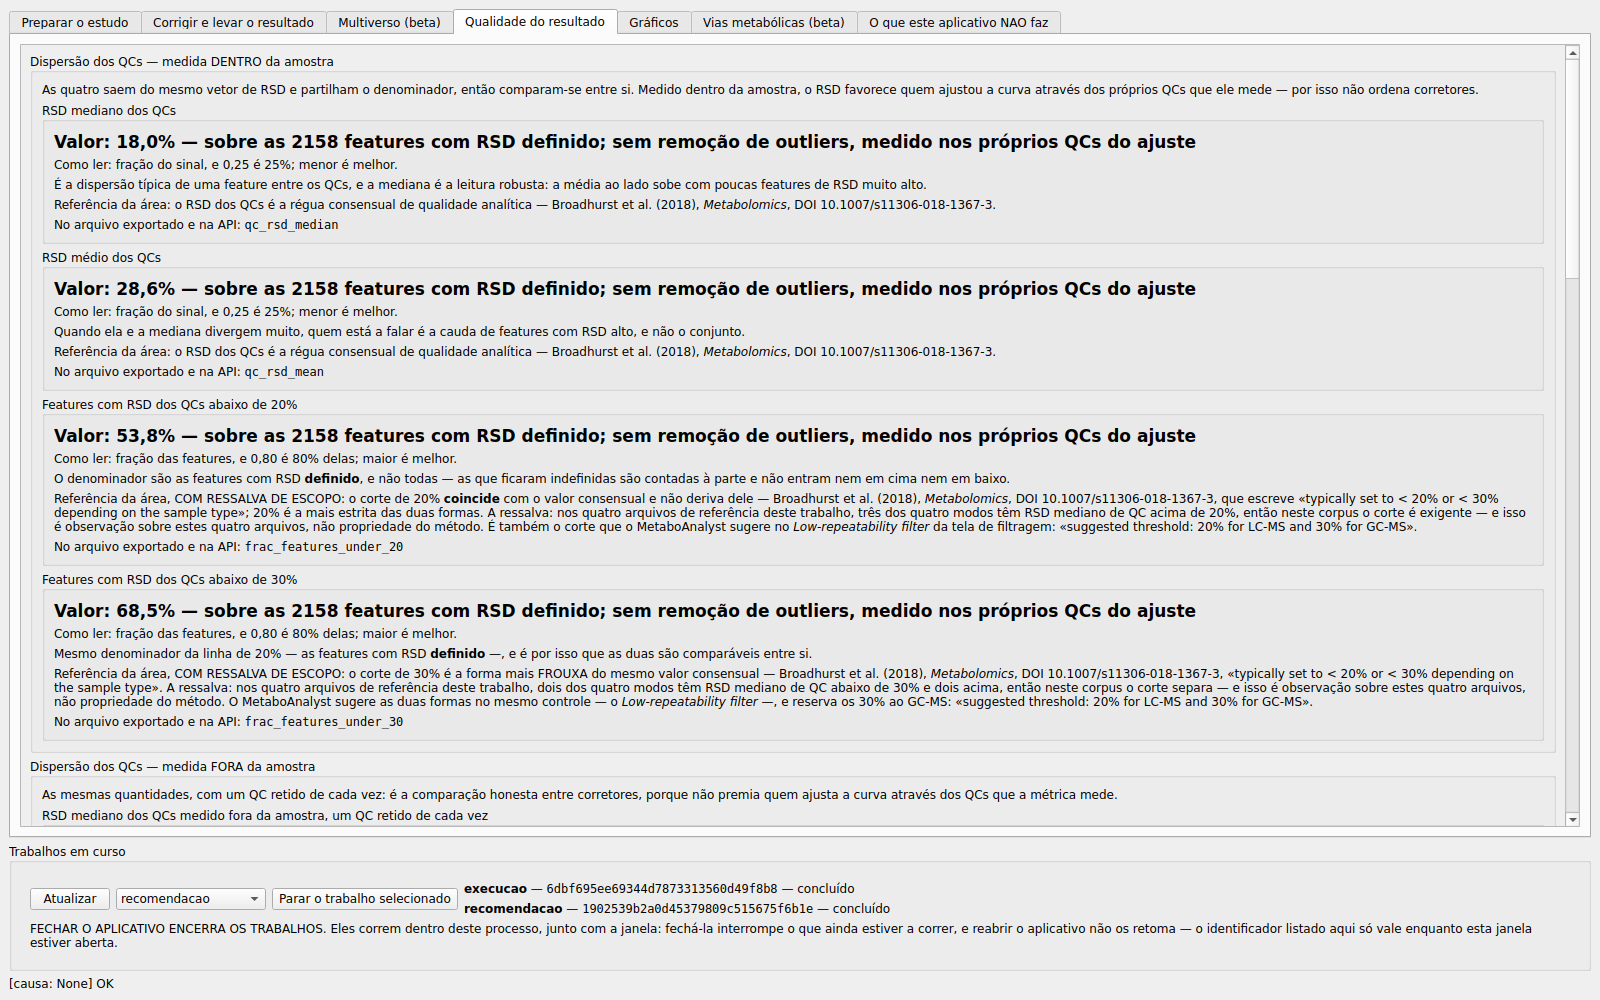
\includegraphics[width=\linewidth]{figs/cap4-aba-qualidade.png}
\fonte{Elaborado pelos autores, com o aplicativo, em 10/11/2026.}
\end{figure}

\begin{figure}[htbp]
\centering
\caption{Aba ``Gráficos'' do aplicativo, com a trajetória dos QCs ao longo da corrida}\label{fig:4-aba-graficos}
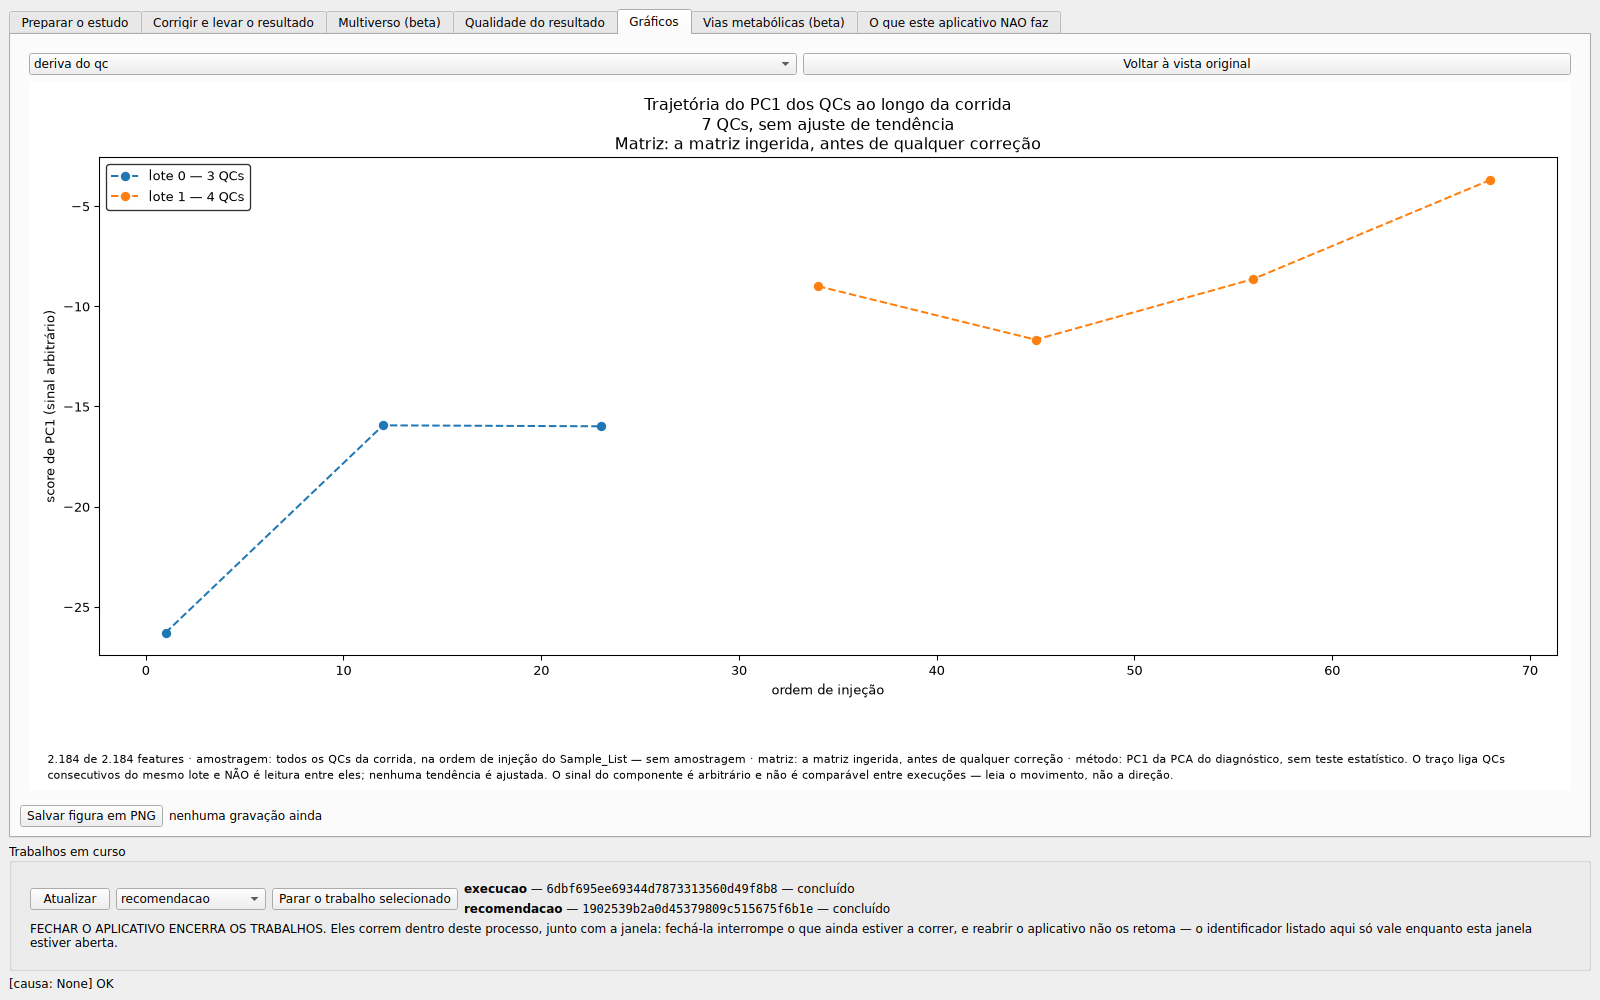
\includegraphics[width=\linewidth]{figs/cap4-aba-graficos.png}
\fonte{Elaborado pelos autores, com o aplicativo, em 10/11/2026.}
\end{figure}

A aba \textit{Preparar o estudo} concentra a seleção dos arquivos de entrada e a verificação das informações necessárias ao processamento. Nesse ponto, o usuário informa a matriz de medições e a lista de amostras correspondentes. A aplicação utiliza essas entradas para associar os valores medidos aos metadados, incluindo a ordem de injeção.

Após a seleção, o usuário pode solicitar a validação dos arquivos. Os problemas identificados são apresentados antes da execução do tratamento, permitindo revisar as inconsistências e corrigir as entradas. Essa posição da validação no fluxo evita que falhas estruturais sejam percebidas apenas durante operações de maior duração.

O diagnóstico acrescenta informações sobre o comportamento da matriz e dos controles de qualidade. Seus resultados auxiliam a escolha do método de correção e a avaliação de possíveis fronteiras de lote. As sugestões produzidas pelo sistema permanecem sujeitas à revisão do profissional.

A aba \textit{Corrigir e levar o resultado} reúne os controles de configuração e execução do processamento. O usuário pode selecionar o corretor e definir as operações posteriores, como filtragem, tratamento de valores ausentes, normalização, transformação e escalonamento. Por padrão, a caixa ``Automático'' vem marcada e aplica o corretor do palpite, medido em 200 \textit{features}; o usuário pode desmarcá-la, comparar os métodos pela medição completa e escolher o corretor.

A configuração aplicada integra o registro da execução. A organização dos controles permite relacionar o resultado aos parâmetros escolhidos, evitando que o processamento seja apresentado como uma operação única cujas decisões internas não possam ser identificadas.

A aba \textit{Qualidade do resultado} apresenta os indicadores utilizados na avaliação do tratamento. As informações são agrupadas por tema, permitindo examinar diferentes aspectos da matriz sem reduzir a qualidade a uma única medida. A apresentação considera o ponto do processamento e as condições em que cada indicador foi calculado.

A aba \textit{Gráficos} disponibiliza as representações visuais dos dados e das análises. O usuário seleciona a figura de interesse e examina aspectos como distribuição dos valores, dispersão dos controles de qualidade, estrutura multivariada e diferenças entre grupos. As figuras também podem ser exportadas para utilização em relatórios e apresentações.

A aba \textit{O que este aplicativo NÃO faz} explicita os limites das funcionalidades. Essa informação integra o fluxo de utilização porque o tratamento computacional de uma matriz não equivale à identificação de compostos, à confirmação de significado biológico ou à validação clínica dos resultados.

A área \textit{Trabalhos em curso} permanece disponível durante a navegação. Ela permite consultar o estado das operações e solicitar o cancelamento dos trabalhos que não precisam continuar. Dessa forma, o acompanhamento não fica restrito à aba em que a execução foi iniciada.

O fluxo principal de utilização pode ser organizado nas seguintes etapas:

\begin{enumerate}
    \item selecionar a matriz de medições e a lista de amostras;
    \item validar os arquivos e revisar os problemas identificados;
    \item examinar o diagnóstico e as sugestões de processamento;
    \item definir o corretor e os parâmetros de pré-processamento;
    \item iniciar a execução e acompanhar seu andamento;
    \item avaliar as métricas e os gráficos disponíveis;
    \item exportar o resultado correspondente ao ponto de processamento desejado.
\end{enumerate}

Essa sequência estabelece uma relação entre preparação, execução e avaliação. A exportação ocorre após a definição do procedimento e a obtenção de seus resultados, permitindo que o profissional examine o tratamento antes de encaminhar os dados às análises seguintes.

\subsection{Apresentação dos resultados e mensagens ao usuário}
\label{subsec:resultados-mensagens}

A apresentação dos resultados busca tornar identificáveis o procedimento aplicado, as medidas calculadas e as condições que limitam sua interpretação. A interface combina informações textuais, indicadores, tabelas e gráficos, utilizando cada representação conforme o tipo de conteúdo.

Os problemas de validação são apresentados com identificação e descrição. A distinção entre erro, aviso e informação permite reconhecer a gravidade da ocorrência e compreender se ela impede o processamento ou exige avaliação adicional. Quando disponível, a localização do problema facilita sua revisão no arquivo de origem.

As mensagens evitam tratar toda ocorrência como uma falha equivalente. Uma entrada incompatível, uma condição que exige atenção e uma operação cancelada possuem significados diferentes e precisam ser representadas de forma correspondente.

As sugestões do sistema são acompanhadas de justificativas, permitindo que o usuário examine a base da escolha antes de aceitá-la ou modificá-la. A possibilidade de sobrescrita mantém o controle metodológico com o profissional e permite registrar sua participação no processo.

A interface distingue o palpite, medido numa amostra de 200 \textit{features}, da medição completa, que aplica os corretores a todas as \textit{features}. Essa separação permite distinguir a sugestão dos resultados medidos sobre a matriz inteira.

As métricas são apresentadas com informações que contextualizam seu significado. A identificação do estimador, da população considerada e do ponto de processamento permite reconhecer o que foi medido. Essa contextualização é necessária porque indicadores com o mesmo nome podem assumir interpretações diferentes conforme o procedimento utilizado.

A organização por temas facilita a leitura do conjunto de medidas. Indicadores de repetibilidade, dispersão e estrutura dos dados são examinados de forma complementar. Uma melhoria isolada não é apresentada como comprovação de que todos os aspectos do tratamento foram aprimorados.

Os resultados das análises multivariadas são acompanhados das informações necessárias à interpretação. No caso de métodos supervisionados, as medidas de validação participam da apresentação, evitando que a separação visual entre grupos seja utilizada isoladamente como evidência de capacidade preditiva.

Os gráficos preservam a identificação dos grupos e dos controles de qualidade quando essas informações participam da análise. Títulos, eixos e legendas indicam as quantidades representadas, permitindo relacionar a figura aos dados utilizados em sua construção.

Quando uma figura não pode ser produzida com as informações disponíveis, a interface apresenta essa condição. A ausência de dados necessários não deve resultar na exibição de uma imagem que sugira uma análise válida ou na manutenção de uma figura pertencente a uma execução anterior.

A apresentação também acompanha o estado dos trabalhos. Uma operação em andamento é diferenciada de uma operação concluída, cancelada ou encerrada com falha. O resultado é disponibilizado de acordo com o desfecho correspondente, mantendo a associação entre a solicitação e o artefato recuperado.

As mensagens sobre cancelamento consideram que a solicitação pode depender de um ponto de verificação do processamento para ser atendida. Por isso, solicitar a interrupção e concluir o cancelamento são condições distintas.

As limitações metodológicas permanecem visíveis ao usuário. O aplicativo trata matrizes de sinais analíticos e fornece recursos de avaliação computacional, mas a interpretação científica exige considerar o desenho do estudo e as evidências disponíveis. A apresentação dos resultados deve preservar essa distinção.

\subsection{Empacotamento e distribuição para Windows}
\label{subsec:empacotamento-windows}

O empacotamento foi realizado com PyInstaller, que reúne o código da aplicação, o interpretador Python, as bibliotecas e os recursos necessários à execução. O pacote resultante utiliza o formato de diretório, contendo o arquivo \texttt{refino.exe} e os componentes que sustentam seu funcionamento.

A distribuição em pasta permite iniciar a aplicação após a extração do arquivo compactado. O usuário não precisa instalar Python, executar comandos de preparação do ambiente ou configurar um servidor de banco de dados para utilizar o fluxo principal.

O executável inicia a interface gráfica e a API interna utilizada para acionar as funcionalidades. A comunicação ocorre em endereço local, e o aplicativo administra a inicialização dos componentes necessários. O banco SQLite atende à persistência sem depender de um serviço externo.

O conteúdo distribuído inclui as bibliotecas numéricas, os componentes da interface e os recursos utilizados na apresentação dos resultados. A seleção dos componentes considera as dependências efetivamente necessárias ao aplicativo, evitando incorporar ao pacote todo o ambiente de desenvolvimento.

O processo de empacotamento exige verificar o comportamento do produto gerado. A execução pelo código-fonte e a execução pelo aplicativo congelado possuem diferenças relacionadas à localização dos recursos, ao carregamento de bibliotecas e à disponibilidade de arquivos auxiliares. Por esse motivo, a verificação considera o funcionamento dentro da própria pasta de distribuição.

Entre os aspectos avaliados estão a abertura da janela, a disponibilidade das funcionalidades, a geração dos artefatos e a apresentação dos gráficos. Essas verificações permitem identificar problemas que não seriam observados apenas pela execução dos testes no ambiente de desenvolvimento.

A apresentação de textos também é considerada no produto empacotado. Mensagens e conteúdos com caracteres acentuados precisam permanecer legíveis no executável, preservando a compreensão das instruções e dos resultados pelo usuário.

O pacote público exclui os arquivos produzidos durante a utilização, incluindo o banco de dados, os registros de execução em arquivo e a pasta de saídas. Esses elementos podem conter informações associadas às amostras e não são necessários para distribuir o programa.

A separação entre aplicação e dados evita que uma cópia utilizada no desenvolvimento seja publicada com resultados ou metadados do laboratório. O material distribuído contém os componentes de software necessários à execução, enquanto os arquivos do estudo são fornecidos e utilizados no contexto apropriado.

A distribuição é acompanhada de instruções de utilização em um arquivo de leitura inicial. Esse material orienta a extração do pacote e a abertura do executável, permitindo que o usuário identifique o ponto de entrada da aplicação.

As versões distribuídas recebem identificação própria e podem ser relacionadas ao estado do código-fonte utilizado em sua geração. A conferência por soma de verificação permite comparar a integridade do arquivo compactado com o artefato produzido no empacotamento.

O aplicativo não utiliza instalador nem assinatura de código. Essas características fazem parte do formato de distribuição adotado e são informadas ao usuário. A utilização ocorre diretamente a partir da pasta extraída, que precisa conter os recursos necessários e permitir as operações locais de escrita realizadas pelo sistema.

\subsection{Repositório do código-fonte}
\label{subsec:repositorio-codigo-fonte}

O código-fonte do MetaRefino é mantido em um repositório com controle de versão Git. O versionamento permite acompanhar as alterações realizadas durante o desenvolvimento e identificar o estado do projeto utilizado na geração de uma versão da aplicação.

O repositório reúne o código da interface, os componentes de processamento, os módulos de persistência, as migrações, os testes e os scripts de empacotamento. Também contém os materiais necessários à compreensão da organização do projeto e à preparação do ambiente de desenvolvimento.

A estrutura separa os componentes por responsabilidade, distinguindo o domínio, as operações científicas, a entrada e saída de arquivos, a persistência e a apresentação. Essa organização facilita a localização das funcionalidades e permite relacionar alterações aos componentes afetados.

Os registros de versão contribuem para a manutenção e a rastreabilidade técnica. Uma versão distribuída pode ser associada a um estado específico do código, permitindo identificar quais alterações estão presentes no executável correspondente.

O código adota a licença GPL-3.0-or-later. A licença do software não abrange automaticamente os dados científicos utilizados no desenvolvimento. Os arquivos pertencentes ao laboratório exigem tratamento separado e não devem ser considerados disponíveis para redistribuição apenas por terem sido utilizados na avaliação da aplicação.

O endereço do repositório do projeto é apresentado a seguir:

\begin{quote}
    \textbf{Repositório do código-fonte:} \url{github.com/NishiyaKN/refino-quimiometrico}
\end{quote}
